%
%%%%%%%%%%%%%%%%%%%%%%%%%%%%%%%%%%%%%%%%%%%%%%%%%%%%%%%%%%%%%%%%%%%%%%%%%%%%%%%%
\chapter{Theoretical background}\label{chap:1}
%%%%%%%%%%%%%%%%%%%%%%%%%%%%%%%%%%%%%%%%%%%%%%%%%%%%%%%%%%%%%%%%%%%%%%%%%%%%%%%%
%
%%%%%%%%%%%%%%%%%%%%%%%%%%%%%%%%%%%%%%%%%%%%%%%%%%%%%%%%%%%%%%%%%%%%%%%%%%%%%%%%
\section{Introduction}\label{sec:intro}
%%%%%%%%%%%%%%%%%%%%%%%%%%%%%%%%%%%%%%%%%%%%%%%%%%%%%%%%%%%%%%%%%%%%%%%%%%%%%%%%
%
Monte Carlo methods comprise many high level concepts as well as manifold
specific algorithms. They all have in common that they make use of randomness to
draw conclusions about statistical quantities. Generally, Monte Carlo methods
are applicable to almost any problem with statistically defined properties.
Therefore it does not come as a surprise that they are commonly used in physics
to describe complex interacting systems with many degrees of freedom. Although
generally applicable and relatively simple to understand and implement, Monte
Carlo methods must not be applied blindly. They are almost always inferior to
more specialized methods and might fail altogether in certain situations. Hence,
careful analysis is absolutely vital for any Monte Carlo method. In theory there
are accurate measures for the applicability of the methods, but in practice it
frequently proves quite delicate to apply those measures correctly.
Unfortunately, pitfalls are often overlooked or even ignored in the literature.
This report focuses on an ab-initio introduction to Monte Carlo methods by
reference to a specific real world example. After developing the theoretical
concepts we actually apply them in great detail to illustrate some common
difficulties.

The concrete physical model deals with a rather recently discovered magnetic
phenomenon, called \newterm{skyrmions}. Since the theoretical prediction of
skyrmions in the eighties by Bogdanov~\cite{bogdanov} based on previous work in
particle physics by Skyrme~\cite{skyrme} and the subsequent experimental
discovery, this configuration has been extensively investigated both by
theorists and experimentalists~\cite{skyrm1, skyrm2, skyrm3, skyrm4, skyrm5,
skyrm6, Milde1076, skyrm8, skyrm9, skyrm10}. Skyrmions have caused a lot of
excitement mostly due to their promising properties that might qualify them as
fast and efficient memory~\cite{switching}. Three-dimensional non-perturbative
classical Monte Carlo methods developed recently~\cite{skyrmionlattice,
Milde1076}, allow us to compute the full finite temperature phase diagram and
explore phase transitions.  The goal of this project was to implement a Monte
Carlo code with the discretized lattice Hamiltonian introduced
in~\cite{skyrmionlattice} and basically reproduce the results discussed there.
In contrast to most work on Monte Carlo methods for spin lattices, we found it
worthwhile to provide a detailed exposition of the algorithms and numerical
aspects.

As a consequence there will be two separate reports. This one focuses on the
algorithmic aspects and Monte Carlo methods in general, while the other one will
go into more detail about the model and discuss physical results. The present
text can serve as a step-by-step introduction on how to write Monte Carlo codes
and discusses associated pitfalls in detail based on a concrete example. All
code is publicly available on GitHub under
\href{https://github.com/nikikilbertus/Sky-MoCa}{\textsf{https://github.com/nikikilbertus/Sky-MoCa}}
and we hope that it will be useful to others.

The report is structured as follows. We briefly introduce the model Hamiltonian
in \secref{sec:model}. In \secref{sec:mctheory} we provide a first high level
overview of Monte Carlo integration and optimization and state some important
results mostly without proofs. \Secref{sec:metropolis} is the core part of this
chapter. We derive and discuss properties of the so called \newterm{Metropolis
algorithm} in quite some detail. Furthermore, practical verification strategies
for Monte Carlo codes in general and the Metropolis algorithm in particular are
treated in \secref{sec:analysis}. \Chapref{chap:2} introduces our implementation
of the algorithm, Sky-MoCa, in \secref{sec:code}. In \secref{sec:results}, we go
through the theoretic verification strategies discussed earlier in a specific
sample simulation using Sky-MoCa. This should give the reader a feeling for what
to expect when writing their own Monte Carlo code. Since the main goal of this
report is to illuminate the methods, we move physical results to the second
paper. Finally, we conclude in \secref{sec:conclusion}.
%
%%%%%%%%%%%%%%%%%%%%%%%%%%%%%%%%%%%%%%%%%%%%%%%%%%%%%%%%%%%%%%%%%%%%%%%%%%%%%%%%
\section{The Spin Lattice Model}\label{sec:model}
%%%%%%%%%%%%%%%%%%%%%%%%%%%%%%%%%%%%%%%%%%%%%%%%%%%%%%%%%%%%%%%%%%%%%%%%%%%%%%%%
%
A common high-level way to think about magnetism in condensed matter is in terms
of complex collective behavior of spins, each of which is associated with a
magnetic moment. Astoundingly, this figuratively simple model is quite powerful
and allows for a thorough explanation of a wide range of phenomena. Let us
consider a three-dimensional lattice with equidistant spacing in each direction.
To each lattice site we attach a spin, represented by an element of the unit
sphere~$S^2$, see \figref{fig:s2}. In the following we will often resort to the
two-dimensional model for illustration purposes, because it is easier to draw on
a two-dimensional surface as illustrated in \figref{fig:lattice}. However, all
computations solely concern the three-dimensional model. Each vertex of the
lattice could for example represent a atom in a solid with a rigid crystal
like structure. Hence the whole lattice can be interpreted as the regular atomic
structure of a cubical piece of solid material.

\begin{figure}
  \centering
  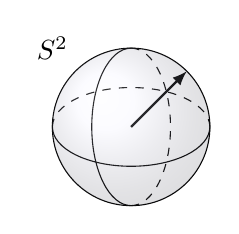
\begin{tikzpicture}
    \draw[->, thick, \select, >=latex] (0,0) -- (45:1cm);
    \draw (-1,0) arc (180:360:1cm and 0.5cm);
    \draw[dashed] (-1,0) arc (180:0:1cm and 0.5cm);
    \draw (0,1) arc (90:270:0.5cm and 1cm);
    \draw[dashed] (0,1) arc (90:-90:0.5cm and 1cm);
    \draw (0,0) circle (1cm);
    \shade[ball color=blue!10!white,opacity=0.20] (0,0) circle (1cm);
    \node at (-1,1) {$S^2$};
  \end{tikzpicture}%
  \caption{We consider three-dimensional spins, \ie{} elements of the unit
  sphere~$S^2$.}
\label{fig:s2}
\end{figure}

\begin{figure}
  \centering
  \begin{tikzpicture}
    \latticeinter{4}
    \begin{scope}[xshift=8cm,yshift=1cm]
      \lattice{4}
    \end{scope}
  \end{tikzpicture}%
  \caption{On the left side we show a two-dimensional spin lattice. Each lattice
  site carries a magnetic moment or spin, represented by an arrow of unit
  length, \ie{}, in the two-dimensional picture, by an element of~$S^1$. The
  neighbors of a lattice site are the ones above, below, left and right in the
  two-dimensional case. The blue squares are the neighbors of the red circle.
  The three-dimensional picture on the right side becomes unclear in a
  two-dimensional drawing rather quickly. Note that the magnetic moments are now
  also three-dimensional, \ie{} elements of the two-dimensional unit
  sphere~$S^2$. In three dimensions each vertex has up to six neighbors.}
\label{fig:lattice}
\end{figure}

We work with a cubic lattice
%
\begin{equation}
  \Sigma := \numlist{1}{N_x} \times \numlist{1}{N_y} \times
  \numlist{1}{N_z} \subset \bN^3 \subset \bR^3\:,
\end{equation}
%
where we interpret~$(i,j,k) \in \Sigma$ as~$i \hx + j \hy + k \hz
\in \bR^3$. Here,~$\hx, \hy, \hz$ are the standard basis vectors of~$\bR^3$.
Note that we can translate the whole lattice by arbitrary integer linear
combinations of the standard basis vectors, thus starting at~$(1,1,1)$ does not
have any physical meaning. It merely corresponds nicely to the numerical
implementation in any~$1$-indexed programming language. At each point~$\r \in
\Sigma$ we attach a spin~$\S_{\r} \in S^2$, resulting in the overall
configuration space
%
\begin{equation}
  \Pi := \prod_{\r \in \Sigma} S^2\:.
\end{equation}
%
Each element of~$\Pi$ consists of~$\abs{\Sigma}=N_x N_y N_z$ spins and thus
describes one possible configuration of the whole system. We refer to the
specific spin at position~$\r \in \Sigma$ by~$\S_{\r} \in S^2$. Note that only
the positions of the spins are discretized, but not explicitly their directions.
In any real implementation there is always a fine grained discretization caused
by the finite number of representable floating point numbers. Discrete vertices
and continuous three-dimensional spins mirror nicely the natural crystal
structure of solids.

In a typical physical simulation one might want to find the ground state of this
system, \ie{} the lowest energy state, for some given external and internal
parameters. Alternatively, we could be interested in macroscopic properties such
as the specific heat or magnetization. Necessarily, we need to define some
notion of energy and also identify some possible parameters for the spin
lattice. Apparently any physical measure of energy must be based on interactions
between the spins within the system or with external fields. Let us elaborate on
some possible interactions. Each of them comes with a constant that can be
interpreted as a weight, \ie{} how much the respective interaction contributes
to the energy with respect to the others. Those material constants can be
treated as free parameters in the simulation.

\subsection{Interactions}

\subsubsection{Ferromagnetic/direct exchange}

The most obvious interaction is the \newterm{ferromagnetic} or \newterm{direct}
exchange. Pictorially speaking, it favors constellations where spins that are
close to each other point into the same direction. A system only interacting
this way will end up in a state where all spins are parallel to each other. The
measure for parallelism of two neighboring spins~$\S_{\r_1}, \S_{\r_2} \in S^2$
can be expressed as
%
\begin{equation}
  -\S_{\r_1} \cdot \S_{\r_2} =
  -\norm{\S_{\r_1}} \norm{\S_{\r_2}} \cos(\alpha) \:,
\end{equation}
%
where~$\alpha$ is the angle between~$\S_{\r_1}$ and~$\S_{\r_2}$. The minus sign
ensures that the energy of two parallel spins is actually smaller than the
energy of two perpendicular or even antiparallel ones. We will always consider
the ferromagnetic exchange to be \newterm{local} or \newterm{short ranged} in
the sense that it only contributes to the energy for adjacent lattice sites, as
shown in \figref{fig:lattice}.

\subsubsection{Interaction with an external field}

Another important and absolutely standard exchange term describes the
interaction of the system with an \newterm{external magnetic field}. Clearly,
every spin tries to align with an external field~$\B$, which we express
mathematically via~$-\B \cdot \S$ for every spin~$\S$ on the lattice. This
contribution is also called the \newterm{Zeeman energy}. It can be misleading to
use terms such as \newterm{non-local} or \newterm{long ranged} for this
exchange, since it is not an interaction between two or more spins within the
system, but affects each lattice site independently in the same fashion.
Naturally, for the external field,~$\B$ itself is the weight or parameter of the
interaction.

\subsubsection{Dipole-dipole interaction}

The \newterm{dipole-dipole interaction} is somewhat more complex, but also much
weaker than the two previous ones. For two spins~$\S_{\r_1}, \S_{\r_2} \in S^2$,
it is given by
%
\begin{equation}
  - {\norm{\r}^{-3}} (3 (\S_{\r_1} \cdot \hat{\r})
  (\S_{\r_2} \cdot \hat{\r}) - \S_{\r_1} \cdot \S_{\r_2})\:,
\end{equation}
%
where~$\r = \r_2 - \r_1$ and~$\hat{\r} = \r / \norm{\r}$ points from the
location of the first spin to the location of the second one. The dipole-dipole
interaction depends on the distance between the two lattice sites as well as the
orientation of the two spins not only relative to each other, but also to the
line connecting them. Moreover, the explicit dependence on the relative position
already indicates that the dipole-dipole interaction is relevant for each pair
of magnetic moments in the system, it is a long ranged interaction. For a
lattice with~$N^3$ vertices the number of pairs scales like~$N^6$. Due to
limited computational resources and its relative weakness, most simulations do
not take the dipole-dipole exchange into account. We will also disregard it
completely in our implementation and further discussion in this report.

\subsubsection{Dzyaloshinskii-Moriya exchange}

In this work we are interested in crystals that lack inversion symmetry, \eg{}
MnSi, and thus exhibit chiral magnets. The missing inversion symmetry gives rise
to the so called \newterm{weak Dzyaloshinskii-Moriya} (DM) coupling. Like the FM
interaction, the DM exchange only contributes for adjacent lattice sites. The
discretized version for two spins~$\S_{\r_1}, \S_{\r_2} \in S^2$ at neighboring
positions~$\r_1, \r_2 \in \Sigma$ reads
%
\begin{equation}
  - (\S_{\r_1} \times \S_{\r_2}) \cdot (\r_2 - \r_1)\:.
\end{equation}
%
Note that~$\r_2 - \r_1$ is normalized by definition for neighboring vertices.
Since the cross product is zero for parallel vectors and maximal for
perpendicular ones, the DM coupling acts against the ferromagnetic interaction
and favors constellations where adjacent spins are perpendicular to each other
in the plane normal to their connecting line.

\subsection{The Hamiltonian}

\subsubsection{Summing up the interactions}

Let us now combine the FM and DM interaction as well as an external magnetic
field to compute the energy for the lattice~$\Sigma$. To this end we add up the
contributions from each spin and for each interaction. For instance, the
external field exchange term simply becomes
%
\begin{equation}\label{Bsum}
  -\sum_{\r \in \Sigma} \S_{\r} \cdot \B\:.
\end{equation}
%

Adding up the terms for the FM interaction with all direct neighbors naively as
in
%
\begin{equation}\label{FMsumnaive}
  -\sum_{\r \in \Sigma} \S_{\r} \cdot (\S_{\r + \hx} + \S_{\r - \hx} +
    \S_{\r + \hy} + \S_{\r - \hx} + \S_{\r + \hz} + \S_{\r - \hz})\:,
\end{equation}
%
poses two problems. First, apparently in this fashion we count the interaction
between some pairs of spins multiple times. If~$\Sigma$ was an infinite grid,
\ie{}~$\Sigma=\bZ^3$, we would count every pair exactly twice and could simply
divide~\eqref{FMsumnaive} by~$2$. However,~$\Sigma$ is finite which leads
to the second more subtle issue. Not every lattice site has a neighbor in each
direction~$\hx, \hy, \hz$. Consider the spin in the lower right corner of the
lattice in \figref{fig:lattice}. The sum in our first naive expression for the
FM interaction~\eqref{FMsumnaive} suggests that we need its right and lower
neighbor, which apparently do not exist. As a consequence, we need to define
some behavior at the boundaries. There are several ways to do this and a
plausible treatment of boundary conditions is a central aspect of many different
areas in scientific computing. It is important to realize that this is not
simply an implementation nuisance that we can get rid off by any means that do
not break the code. Various boundary conditions represent different physical
systems and can significantly alter the results of a simulation.

\subsubsection{Boundary conditions}

In many cases the desired simulation volume is an infinite space, or at least so
large compared to all internal length scales that it is practically infinite. On
physical computing machines we are always limited to finite grids. The most
obvious way for finite systems is to set all spins outside of~$\Sigma$ to zero,
\ie{}~$\S_\r = 0$ for all~$\r \in \bZ^3 \setminus \Sigma$. Consequently the
lattice sites on the boundary have less neighbors to interact with. This is
called an \newterm{open boundary}. Open boundaries are often undesirable,
because they heavily impact the physical behavior. In our example, a magnetic
moment at the boundary is less effected by the FM and DM interaction, simply
because it has less neighbors. However, the external field still has the same
impact on a boundary spin as on any other vertex. This imbalance leads to
polarized magnetic moments at the boundaries, \ie{} they tend to all point in
the direction of the external magnetic field~$\B$ to maximize their Zeeman
energy.

One common way to get out of this dilemma is to implement \newterm{periodic
boundary conditions}. We think of our lattice as a finite box of volume~$L^3$
for~$L\in \bRp$ and simply replicate that box infinitely many times to fill the
whole space, see \figref{fig:periodic} for a two-dimensional illustration. In
practice, we will access the lattice sites by indexing a three-dimensional array
with indices~$(i,j,k)\in\Sigma$. Whenever the algorithm tries to index out of
bounds, \eg{} requests~$j=N_y + 1$, we simply use~$j=1$ again. For~$i=0$ we
use~$i=N_x$,~$k=N_z+2$ is replaced by~$k=2$ and so on. In general, this behavior
can be achieved by always working with the indices
%
\begin{equation}\label{periodicindices}
  ((i-1 \mod N_x) + 1, (j-1 \mod N_y) + 1, (k-1 \mod N_z) + 1) \in \Sigma
\end{equation}
%
whenever the algorithm requests the spin at position~$(i,j,k) \in \bZ^3$. By
construction, those new indices always lie in~$\Sigma$. We can now
unproblematically include spins at officially non-existing positions in our
mathematical expressions, implicitly assuming that those are being wrapped
around periodically to positions within the original lattice. This way every
vertex has the same number of neighbors and we do not observe spurious boundary
effects. In this report, we will only employ periodic boundary conditions in all
three directions using~\eqref{periodicindices}. For other scenarios we kept the
possibility of opening up the boundaries in one direction in our implementation.
This solves the issue of missing neighbors, which we encountered
in~\eqref{FMsumnaive}.

\begin{figure}
  \centering
  \begin{tikzpicture}
    \periodic{}
  \end{tikzpicture}
  \caption{We illustrate periodic boundary conditions for a
  two-dimensional~$4\times4$ grid. The simulation volume stored in memory is
  given by the shaded square in the middle. This square is copied over and over
  again in all directions as indicated by the surrounding lattice sites. Note
  how the four boundaries of the square keep their orientation throughout that
  copying procedure. While it appears like we have filled an infinite space, all
  red squares are identified, because they are represented internally by only
  one vertex in the central square. The same holds true for the green pentagons
  of course. If the code tries to fetch the spin at the right neighbor of the
  green pentagon in the central square, we can instead pick the right neighbor
  of \emph{any} green pentagon. One of those will always lie in the center
  square and is thus available in memory.}
\label{fig:periodic}
\end{figure}

\subsubsection{Combining all interactions}

Now that we have established a well defined behavior at the boundary, we can
also tackle the problem of counting interactions multiple times. For periodic
boundary conditions we could divide expression~\eqref{FMsumnaive} by~$2$. In the
implementation we do not want to actually carry out redundant computations, thus
we work with
%
\begin{equation}\label{FMsum}
  -\sum_{\r \in \Sigma} \S_{\r} \cdot
    (\S_{\r + \hx} + \S_{\r + \hy} + \S_{\r + \hz})\:.
\end{equation}
%
It is worth convincing oneself that in this expression, assuming open or
periodic boundary conditions, every pair of neighboring lattice sites is
included exactly once.

Finally, the overall DM energy is analogously
%
\begin{equation}\label{DMsum}
  -\sum_{\r \in \Sigma} ((\S_{\r} \times \S_{\r + \hx}) \cdot \hx +
    (\S_{\r} \times \S_{\r + \hy}) \cdot \hy +
    (\S_{\r} \times \S_{\r + \hz}) \cdot \hz)\:.
\end{equation}
%
Everything we discussed about boundary conditions for the FM exchange also holds
true for the DM interaction. Adding up all
interactions~\eqref{Bsum}, \eqref{FMsum} and~\eqref{DMsum}, we obtain the
Hamiltonian, \ie{} the energy of the system in a given configuration~$\pi \in
\Pi$
%
\begin{align}\label{hamiltonian}
  H(\pi) = &-\sum_{\r \in \Sigma}\biggl(\S_{\r} \cdot \B +
      J\; \S_{\r} \cdot (\S_{\r+\hx} + \S_{\r+\hy} + \S_{\r+\hz})\nonumber \\
      &+ K\; (\S_{\r} \times \S_{\r+\hx} \cdot \hx +
            \S_{\r} \times \S_{\r+\hy} \cdot \hy +
            \S_{\r} \times \S_{\r+\hz} \cdot \hz)\biggr)\:.
\end{align}
%
The parameters~$J$,~$K$ and~$\B$ are sometimes used synonymously for the
ferromagnetic, the Dzyaloshinskii-Moriya and the external field interaction
terms respectively. The physical behavior of the system strongly depends on
these freely adjustable parameters. For a given set of parameters and at zero
temperature we expect the system to settle in the ground state, which can be
defined as the lowest energy configuration
%
\begin{equation}\label{objective}
  \argmin_{\pi \in \Pi} H(\pi)\:.
\end{equation}
%

\subsubsection{Anisotropy}

In~\eqref{hamiltonian} we have collected all interactions on the lattice. Those
originally stem from a continuous model. Therefore we have to expect
discretization errors. In particular, the transition to a finite cubical
lattice introduces anisotropies that are absent in the original continuum model.
Buhrandt and Fritz show in~\cite{skyrmionlattice} that we can partly compensate
for those disruptive anisotropies by adding next-nearest neighbor interactions
to the Hamiltonian. The optimal choice to render higher order deviations from
the continuous model as small as possible is
%
\begin{align}\label{hamiltonianfix}
  H'(\pi) = & \sum_{\r \in \Sigma} \biggl(
  \frac{J}{16} \S_{\r} \cdot (\S_{\r+2\hx} + \S_{\r+2\hy} + \S_{\r+2\hz})\nonumber \\
  &+ \frac{K}{8} (\S_{\r} \times \S_{\r+2\hx} \cdot \hx +
        \S_{\r} \times \S_{\r+2\hy} \cdot \hy +
        \S_{\r} \times \S_{\r+2\hz} \cdot \hz)\biggr)\:.
\end{align}
%
The Hamiltonian used in the simulation is then~$H + H'$. Note that~$H'$ has the
same structure of the FM and DM term of~$H$, but enters with smaller constants
and opposite sign. Thus it complements the nearest neighbor exchange by a
directly related next-nearest neighbor interaction term. Adding next-nearest
neighbor interactions makes a big difference computationally, but is handled
analogously to the nearest neighbor interactions, see \figref{fig:interact}.
Periodic and open boundaries still work precisely the same way and are already
taken care of by~\eqref{periodicindices}.

\begin{figure}
  \centering
  \begin{tikzpicture}
    \latticeinternn{5}
  \end{tikzpicture}%
  \caption{We select a spin at position~$\r \in \Sigma$ (red circle) and show
  its nearest neighbors as blue squares and the next-nearest neighbors as green
  pentagons. Note that although the diagonally adjacent vertices are closer
  to~$\r$ than the next-nearest neighbors, they are not included in any
  exchange terms of the Hamiltonian.}
\label{fig:interact}
\end{figure}

\subsection{A note on parameter values}

Recall that there is a great conflict of interest between the FM and the DM
interactions. While the FM term in the Hamiltonian is minimal when all spins are
parallel to each other, the DM term favors a configuration where neighboring
spins are orthogonal. The specific compromise between those effects depends
mostly on their respective strengths~$J$ and~$K$. In reality the direct
interaction~$J$ is much stronger and one typically encounters helical or conical
structures with long modulation periods for zero or small external fields
respectively. For example in MnSi the spins wind around a given modulation axis
only once per roughly~$40$ lattice spacings. By tuning the ratio~$J/K$ we can
set the periodicity. For a period of~$N$ lattice sites, we have to set~$J/K$
to~$1/\tan(2\pi / N)$. In all our simulations we chose~$J=1$ and~$K=\tan(2\pi /
10)$, \ie{} one full modulation every~$10$ vertices. Because~$K=\tan(2\pi /
10)\approx 0.73$ is not much smaller than~$J=1$ we cannot directly model known
chiral magnets such as MnSi in our simulation. However, larger periodicities
would require much larger grids and thus be computationally infeasible.
Moreover, we let the external magnetic field point in the~$\hz$
direction~$\B=(0,0,B)$ and only keep~$B$ as a free scalar parameter.

We can fix one of the parameters, in this case~$J$, arbitrarily and then work in
abstract lattice units. A computer can only deal with dimensionless numbers and
in numerical simulations one often makes convenient, but arbitrary choices.
It is then sometimes quite difficult to translate the results back to physically
meaningful values.

The alert reader might have realized that so far our model does not contain any
thermal energy. When talking about magnetism, temperature typically has a strong
influence on the physical properties of various materials. However, thermal
energy cannot be accounted for by an additional term in the Hamiltonian. Our
intuition tells us that thermal energy is intrinsically of dynamic nature, thus
cannot be captured sensibly in a single static spin configuration. Thermodynamic
observables are statistical properties of an ever evolving underlying system. In
fact we will account for temperature not in the Hamiltonian but via the
Metropolis algorithm, which we describe in \secref{sec:metropolis}, where the
dynamic and statistical nature of thermodynamics will become apparent.

\subsection{Summary}

In this section we have set up our model, which we want to summarize briefly. We
work on the lattice
%
\begin{equation}
  \Sigma := \numlist{1}{N_x} \times \numlist{1}{N_y} \times
  \numlist{1}{N_z} \subset \bN^3 \subset \bR^3\:
\end{equation}
%
and attach a spin~$\S_{\r} \in S^2$ to each lattice site~$\r \in \Sigma$. This
yields the configuration space
%
\begin{equation}
  \Pi := \prod_{\r \in \Sigma} S^2\:.
\end{equation}
%
On~$\Pi$ we define the Hamiltonian~$H+H'$ from~\eqref{hamiltonian}
and~\eqref{hamiltonianfix} where we implement periodic (or partially open)
boundary conditions. The parameters~$J=1$ and~$K=\tan(2\pi / 10)$ of the FM and
DM interaction are fixed, which leaves us only with the magnetic field in
the~$\hz$ direction~$B$ as a free parameter. In the next section we will
introduce the temperature as a second adjustable quantity. Instead of finding
the energy minimizing configuration as stated in~\eqref{objective} at zero
temperature, we now seek to evaluate prominent observables such as the
magnetization or specific heat of the system for given values of~$B$ and~$T$. As
mentioned before, we cannot expect to compute such macroscopic properties from a
single static configuration~$\pi \in \Pi$ due to thermal effects. Before we go
into statistical physics, let us present a first primer on general Monte Carlo
methods.
%
%%%%%%%%%%%%%%%%%%%%%%%%%%%%%%%%%%%%%%%%%%%%%%%%%%%%%%%%%%%%%%%%%%%%%%%%%%%%%%%%
\section{General Monte Carlo methods}\label{sec:mctheory}
%%%%%%%%%%%%%%%%%%%%%%%%%%%%%%%%%%%%%%%%%%%%%%%%%%%%%%%%%%%%%%%%%%%%%%%%%%%%%%%%
%
Now that we have clearly stated the model, let us start going into algorithmic
techniques. Monte Carlo methods stand for a broad class of numerical algorithms
that are based on some sort of repeated random sampling. The term was coined by
the casinos in Monte Carlo, where gamblers bet on the outcome of random
processes. It is hard to formulate a more specific feature that all Monte Carlo
algorithms have in common. Most often, Monte Carlo techniques are used for
optimization, integration or sampling probability distributions. Our specific
problem contains a mixture of all three fields, arguably with the main focus on
integration.

Before we describe the Metropolis algorithm in detail, we have to issue a
warning. While Monte Carlo methods are generally easy to implement and are
sometimes even applied blindly to virtually any problem, they are almost always
hopelessly inferior to specialized techniques in terms of accuracy and
efficiency. They should be the last resort after everything else has failed. We
will reason about this in the following subsections. Let us start out with a
general description of Monte Carlo integration and optimization.

The remainder of this chapter is based on a collection of different overview
articles~\cite{mc09, mc14, mc00} as well as comprehensive books on Monte Carlo
methods in statistical physics~\cite{mcbook, optinphysics}.

\subsection{Integration}\label{integration}

\subsubsection{Overview and comparison of integration methods}

The oldest and most naive numerical integration methods make use of
interpolating functions. They sample the integrand at a fixed finite number of
base points in the domain and approximate the integrand by an interpolation that
is easy to integrate. Consider for example the trapezoidal rule. It samples the
integrand on a homogeneous grid and approximates it by a piecewise linear
function between the grid vertices, see \figref{fig:int}. The integral of a
piecewise linear function is easily computed by adding up the areas of the
trapezoids underneath the curve. The larger the number of base points, \ie{} the
smaller the grid spacing, the more accurate is the result for sufficiently well
behaved integrands. The important aspect here is that for a given integration
rule and a given number of base points the choice of nodal points in the domain
is completely deterministic.

More sophisticated routines refine the grid of base points iteratively in
regions, where the error does not meet certain accuracy and precision goals. But
even such \newterm{adaptive} methods have fixed rules how the new samples have
to be chosen. Typically that determinism brings great advantage, because one can
prove optimality results and certain error bounds for wise choices of base
points.

In contrast, Monte Carlo techniques draw the samples randomly from some
probability distribution. The general idea is illustrated by the one-dimensional
example of a real-valued function~$f$ on the interval~$[0,1] \subset \bR$. From
the definition of the expectation value we have
%
\begin{equation}\label{mcsimple}
  \int_0^1 f(x) \sucd{x} = E_{\cU_{[0,1]}}(f)\:,
\end{equation}
%
where~$E_{\cU_{[0,1]}}$ is simply the expectation value over the uniform
distribution~$\cU$ on the interval~$[0,1]$. The expectation value can be
approximated by averaging~$f$ over~$N \in \bN$ independent samples~${x_i}$
of a~$\cU_{[0,1]}$ distributed random variable
%
\begin{equation}\label{evapprox}
  E_{\cU_{[0,1]}}(f) \approx \frac{1}{N} \sum_{i=1}^N f(x_i)
\end{equation}
%
and thus
%
\begin{equation}\label{mcsapprox}
  \int_0^1 f(x) \sucd{x} \approx \frac{1}{N} \sum_{i=1}^N f(x_i)\:.
\end{equation}

Both paradigms, the trapezoidal rule as well as the Monte Carlo sampling, are
illustrated for a simple one-dimensional function in the top row
of~\figref{fig:int}. In this one-dimensional scenario the Monte Carlo
integration is absolutely not competitive. Even the crude trapezoidal rule will
easily outperform it in terms of accuracy, precision and also efficiency for any
given number of base points~$N$. It turns out that the error of the trapezoidal
rule scales like~$1/N^2$. Piecewise quadratic approximation, called Simpon's
rule or Kepler rule, already brings the error down to~$\sim 1/N^4$. Hence these
methods converge extremely fast for suitable integrands. Keep in mind that we
are talking about the simplest rules imaginable which are hardly ever used in
practice. State of the art integration methods are far more sophisticated
with still better convergence properties for a certain classes of functions.

However, to exploit the full potential of specialized integration routines one
still has to have some idea of what the integrand looks like. Periodic functions
call for other routines than slightly singular functions with strongly localized
features for instance. Furthermore, even adaptive rules require to at least
crudely sample the whole integration domain. In high-dimensional integrals they
easily fall victim to the curse of dimension. For example, imagine we want to
compute a ten-dimensional integral. Even a coarse first grid of ten base points
in each direction requires~$10^{10}$ function evaluations. For a complex
integrand that requires hundreds or thousands of floating point operations per
evaluation, even that initial sampling exceeds the capacities of a typical
privately owned computer. Once we try to refine the grid by say a factor of~$2$
in each dimension we get into real trouble, since the number of base points
consequently increases by a factor of thousand, rendering most direct
integration routines infeasible even for the fastest computers available. Let us
contrast these insights with the workings and errors of Monte Carlo integration.

\subsubsection{Error of Monte Carlo integration}

First of all, the law of large numbers ensures that the
approximation~\eqref{evapprox} converges for large~$N$
%
\begin{equation}
  \lim_{N \to \infty} \frac{1}{N} \sum_{i = 1}^N f(x_i) = E_{\cU_{[0,1]}}(f)\:.
\end{equation}
%
However, it is important to know how fast it converges, \ie{} how large the
error is. Let us henceforth use~$I$ and~$\hat{I}$ for the exact and approximate
values of the integral
%
\begin{equation}
  I := \int_0^1 f(x) \sucd{x} \qqtxtqq{and}
  \hat{I} := \frac{1}{N} \sum_{i=1}^N f(x_i)\:.
\end{equation}
%
We define the variance of~$f$ by
%
\begin{equation}
  \sigma^2(f) = \int_0^1 (f(x) - I)^2 \sucd{x}\:.
\end{equation}
%
To measure the error in~$\hat{I}$ we consider the~$x_i$ independently
identically distributed random variables with distribution~$\cU_{[0,1]}$. One
can then show that the variance of the Monte Carlo estimate is
%
\begin{equation}\label{mcerror}
  E_{x_1, \dots , x_N}\bigl((\hat{I} - I)^2\bigr) =
  \int_0^1 \pred{x_1} \cdots \int_0^1 \pred{x_N}
  \biggl(\frac{1}{N} \sum_{i=1}^N f(x_i) - I\biggr)^2 =
  \frac{\sigma^2(f)}{N}\:.
\end{equation}

What this tells us is that the average error we make in the Monte Carlo
integration is~$\sigma(f)/\sqrt{N}$. It is important to realize that with truly
random numbers, each separate run of the same Monte Carlo integration will
generally yield different results. For any single one of them the error could be
much larger than~$\sigma(f)/\sqrt{N}$, but for infinitely many runs the average
of all observed errors will always average to the standard deviation of~$f$
divided by~$\sqrt{N}$. By increasing the number of samples we can only bound the
probability of being far off. In stark contrast, interpolation methods like the
trapezoidal rule actually allow for strict absolute upper bounds of the error
for any function meeting certain differentiability criteria.

The single most important result of Monte Carlo integration is that the factor
of~$\sqrt{N}$ is independent of the dimension of the integration domain. This
tells us that even in a~$10^3$ dimensional integration, where interpolation and
adaptive methods would fail straightaway, we can be sure that the average error
scales like~$1/\sqrt{N}$, where~$N$ is the number of samples. This is the key
justification for the use of Monte Carlo methods. Keep in mind, however, that a
convergence rate of~$1/\sqrt{N}$ is tantalizingly slow compared to what we are
used from other numerical algorithms. For example, consider the integral
%
\begin{equation}
  I := \int_0^1 e^{-x} \sucd{x}\:.
\end{equation}
%
Assume we want the error~$\sigma (e^{-x}) / \sqrt{N}$ to be smaller
than~$5 \cdot 10^{-4}$. We compute
%
\begin{equation}\label{sigmaexp}
  \sigma (e^{-x}) =
    \sqrt{E_{\cU_{[0,1]}}(e^{-2 x}) - E_{\cU_{[0,1]}}(e^{-x})^2} =
    0.18098\ldots \:,
\end{equation}
%
which leads to a minimal~$N$ of roughly~$2\cdot10^5$ to achieve our accuracy
goal. We need a couple hundred thousand function evaluations for a moderate
error in a simple and well behaved integral. For comparison, the
trapezoidal rule reaches the same error for about~$15$ base points, see the
second row of \figref{fig:int}, where we show only~$7$ base points for
illustration purposes.

\subsubsection{Importance sampling}

While the~$N$ dependence in the error of Monte Carlo integration is certainly
more important, because it is the one we have full control over, it pays off to
also elaborate on the standard deviation of the integrand~$\sigma(f)$. Although
the integrand is usually fixed by the problem, there are some tricks to improve
the error by decreasing the variance of the integrand. Let us start from a
generic integral
%
\begin{equation}
  \int_{\Omega \subset \bR^n} f(x) \sucd{\lambda}^n(x)\:,
\end{equation}
%
where~$\lambda^n$ is the ordinary Lebesgue measure on~$\bR^n$. Next, let us
rewrite this as
%
\begin{equation}
  \int_{\Omega \subset \bR^n} f(x) \sucd{\lambda}^n(x) =
    \int_{\Omega \subset \bR^n} \frac{f(x)}{p(x)} p(x) \sucd{\lambda}^n(x) =
    \int_{\Omega \subset \bR^n} \frac{f(x)}{p(x)} \sucd{\mu}(x) =
    E_{p}\biggl(\frac{f(x)}{p(x)}\biggr) \:,
\end{equation}
%
where~$p$ is the probability density function of some measure~$\mu$ on~$\Omega$
with respect to the Lebesgue measure. The expectation value~$E_p$ is with
respect to this measure. Since we have changed the integration measure, we can
now approximate the integral by
%
\begin{equation}
  \int_{\Omega \subset \bR^n} f(x) \sucd{\lambda}^n(x) \approx
  \frac{\lambda^n(\Omega)}{N} \sum_{i=1}^N \frac{f(x_i^p)}{p(x_i^p)}\:,
\end{equation}
%
where the~$x_i^p$ are now independent samples from the probability distribution
induced by~$p$. The key point is that the error estimate is unaffected by the
distribution we draw the samples from and is thus given by
%
\begin{equation}
  \frac{\sigma(f/p)}{\sqrt{N}} \:.
\end{equation}
%
While we cannot change the standard deviation of~$f$, we can now try to
minimize the variance of the ratio~$f/p$ by choosing~$p$ wisely. An optimal
choice would mean~$f/p = \const$. This shows that~$p$ should be large/small
where~$f$ is large/small, which makes sense intuitively. We concentrate the
samples in regions where the contributions to the integral are large. Regions
where~$f$ is insignificantly small will only be sampled sparsely. Therefore we
call this procedure \newterm{importance sampling}.

For this method to work in practice, one needs to be able to efficiently sample
the distribution induced by~$p$. In general this is a difficult task and a lot
of research has gone into the development of good pseudo random number
generators following arbitrary probability distributions. Moreover, Monte Carlo
integration is typically used precisely when we do not know much about~$f$,
hence cannot choose~$p$ adequately upfront.

There are algorithms based on importance sampling, for example VEGAS, that
update~$p$ in real time during the integration to concentrate on important
regions. However, it turns out that many integrals that come up in physics,
particularly in statistical physics as we will see later, already come in the
form
%
\begin{equation}\label{probform}
  \int_{\Omega \subset \bR^n} f(x) p(x) \sucd{\lambda}^n(x)\:,
\end{equation}
%
where~$p$ is a probability density function of some measure~$\mu$ on~$\Omega$.
In this case we can directly rewrite the integral as
%
\begin{equation}
  \int_{\Omega \subset \bR^n} f(x) \sucd{\mu}(x) \approx
  \frac{\lambda^n(\Omega)}{N} \sum_{i=1}^N {f(x_i^p)}\:.
\end{equation}
%
Usually~$\sigma(f)$ is smaller than~$\sigma(f\cdot p)$ and as long as we can
sample~$p$ efficiently, we can improve the error for fixed~$N$.

Let us illustrate importance sampling with an example. On the right side of the
second row of \figref{fig:int} we plot the function~$e^{-x}$ and some
uniformly distributed random sample points for ordinary Monte Carlo integration.
The bulk of the area under the curve is on the left, while the long exponential
tail can practically be neglected. However, many of our uniformly chosen samples
fall into the right half, where the function is basically zero. At the same
time we scarcely sample the important region. The rather large variation
of~$e^{-x}$ leads to big errors as we have discovered in~\eqref{sigmaexp}.
Fortunately, with the right normalization~$e^{-x}$ is a probability density
function that can be sampled efficiently on a computer. The integral~$\int_0^1
e^{-x} \sucd{x}$ is of the form~\eqref{probform} with
%
\begin{equation}
  f(x) =\frac{e}{e-1} \qqtxtqq{and} p(x) =\frac{e^{1-x}}{e-1}\:.
\end{equation}
%
In this case the Monte Carlo approximation becomes trivial
%
\begin{equation}
  \frac{1}{N} \sum_{i=1}^N f(x_i^p) = \frac{1}{N} \sum_{i=1}^N \frac{e}{e-1} =
  \frac{e}{e-1} \:,
\end{equation}
%
which is the exact value of the integral, see last row of \figref{fig:int}. In
this simplified case the integrand itself is up to a normalization constant a
probability density function on~$[0,1]$. The function~$f$ that is left as an
integrand is constant, thus has vanishing variance and a single sample is enough
to get the error down to zero. Hence we already computed the integral exactly by
finding the normalization constant for~$p$. In real use cases the function~$f$
would not be constant and we would have to collect more than just one sample for
a reasonable estimate.

\begin{figure}[H]
  \centering
  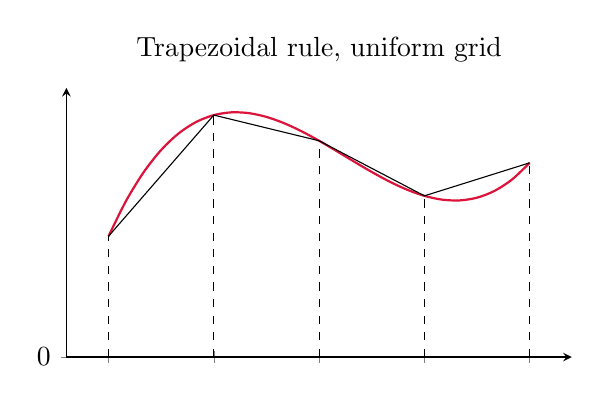
\begin{tikzpicture}[declare function={f=100 - x - 6*x^2 + x^3;}]
    \begin{axis}[
        width=8cm,
        height=5cm,
        ymin=0,
        axis lines=left,
        enlarge y limits=upper,
        enlarge x limits,
        ytick={0},
        xticklabels={,,},
        domain=-2.5:5.5,
        xtick={-2.5, -0.5, ..., 5.5},
        title={Trapezoidal rule, uniform grid},
      ]
      \addplot[thick, Crimson, smooth] {f};
      \addplot[dashed, samples=5, ycomb] {f};
      \addplot[samples=5] {f};
    \end{axis}
  \end{tikzpicture}%
  \hspace{1cm}
  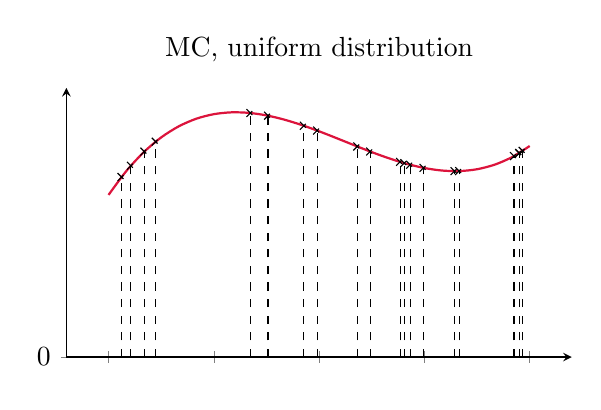
\begin{tikzpicture}[declare function={f=150 - x - 6*x^2 + x^3;}]
    \begin{axis}[
        width=8cm,
        height=5cm,
        ymin=0,
        axis lines=left,
        enlarge y limits=upper,
        enlarge x limits,
        ytick={0},
        xticklabels={,,},
        domain=-2.5:5.5,
        xtick={-2.5, -0.5, ..., 5.5},
        title={MC, uniform distribution},
      ]
      \addplot[thick, Crimson, smooth] {f};
      \addplot[dashed, mark=x, samples at={3.48308, 5.29824, 1.20917,-1.60499,
      3.03779, 1.46106, 3.22893, 4.07112, 2.2248, 4.15928, 5.2014,-2.25321,
      5.30407, 0.19369,-1.81973, 2.46947,-2.07559, 3.11756, 5.36544, 0.529774},
      ycomb] {f};
    \end{axis}
  \end{tikzpicture}%
  \\[1cm]
  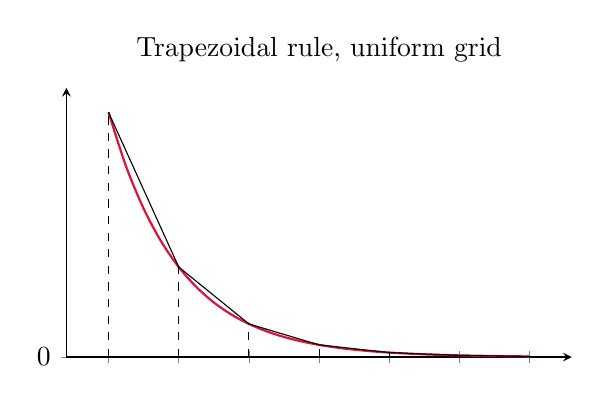
\begin{tikzpicture}[declare function={f=exp(-x);}]
    \begin{axis}[
        width=8cm,
        height=5cm,
        ymin=0,
        axis lines=left,
        enlarge y limits=upper,
        enlarge x limits,
        ytick={0},
        xticklabels={,,},
        domain=0:6,
        xtick={0,...,6},
        title={Trapezoidal rule, uniform grid},
      ]
      \addplot[thick, Crimson, smooth] {f};
      \addplot[dashed, samples=7, ycomb] {f};
      \addplot[samples=7] {f};
    \end{axis}
  \end{tikzpicture}%
  \hspace{1cm}
  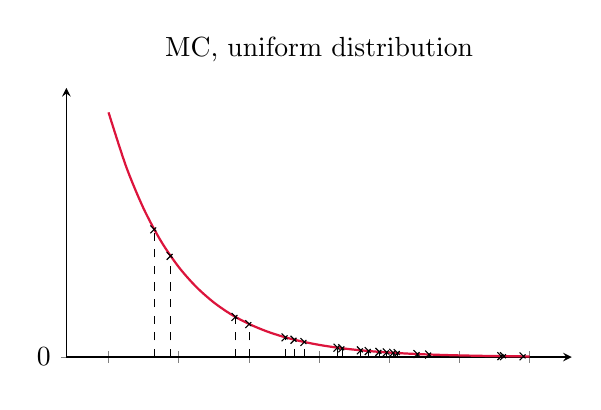
\begin{tikzpicture}[declare function={f=exp(-x);}]
    \begin{axis}[
        width=8cm,
        height=5cm,
        ymin=0,
        axis lines=left,
        enlarge y limits=upper,
        enlarge x limits,
        ytick={0},
        xticklabels={,,},
        domain=0:6,
        xtick={0,...,6},
        title={MC, uniform distribution},
      ]
      \addplot[thick, Crimson, smooth] {f};
      \addplot[dashed, mark=x, samples at={2.79019, 3.26148, 0.650803, 5.91188,
      5.63303, 2.00519, 3.33023, 4.05605, 4.11961, 5.59612, 3.85836, 0.883656,
      3.70697, 2.64962, 1.80842, 2.52199, 4.56677, 3.59437, 4.40159, 3.96445},
      ycomb] {f};
    \end{axis}
  \end{tikzpicture}%
  \\[1cm]
  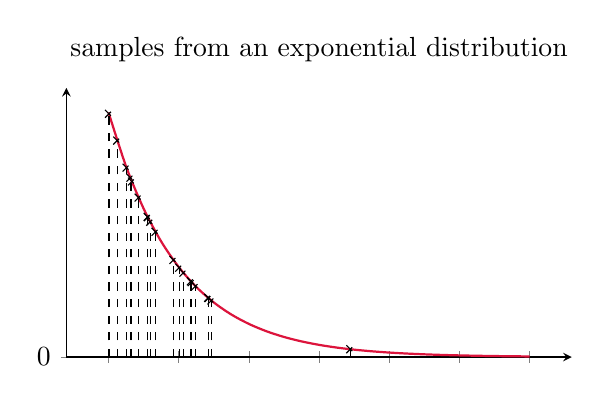
\begin{tikzpicture}[declare function={f=exp(-x);}]
    \begin{axis}[
        width=8cm,
        height=5cm,
        ymin=0,
        axis lines=left,
        enlarge y limits=upper,
        enlarge x limits,
        ytick={0},
        xticklabels={,,},
        domain=0:6,
        xtick={0,...,6},
        title={samples from an exponential distribution},
      ]
      \addplot[thick, Crimson, smooth] {f};
      \addplot[dashed, mark=x, samples at={1.17301, 0.559973, 0.256368, 1.00665,
      1.23844, 0.00605024, 3.44436, 0.122949, 0.311557, 0.428481, 1.06569,
      1.4651, 0.669611, 1.18508, 1.41826, 0.332201, 0.557094, 1.42344, 0.924603,
      0.593438}, ycomb] {f};
    \end{axis}
  \end{tikzpicture}%
  \caption{We show the basic principle of the trapezoidal rule in the left
  column and Monte Carlo integration in the right column. In the top row we
  consider some arbitrary function and draw from a uniform distribution in the
  Monte Carlo integration. In the second row we integrate the
  function~$e^{-x}$. While sampling uniformly yields a big error due to the
  large variation of the exponential function, we can instead draw our samples
  according to an exponential distribution as shown in the bottom center plot.}
\label{fig:int}
\end{figure}

\subsubsection{Jackknife}

While the theoretic prediction for the error in a Monte Carlo integration of the
function~$f$ with~$N$ random samples is given by~$\sigma(f) / \sqrt{N}$, we
cannot compute this quantity in practice. Usually one does not have access
to~$\sigma(f)$. Instead, one typically employs a procedure called
\newterm{jackknife} to estimate the error. Given the samples~$f_i$ for~$i \in
\numlist{1}{N}$, we compute the mean
%
\begin{equation}
  \overline{f} := \frac{1}{N} \sum_{i=1}^N f_i
\end{equation}
%
and define
%
\begin{equation}
  \overline{f}_i := \frac{1}{N-1} \sum_{j=1, j\ne i}^N f_j \:,
\end{equation}
%
for all~$i \in \numlist{1}{N}$. The quantity~$\overline{f}_i$ is the mean of all
samples except the~$i$-th one. An estimate of the variance of the original
estimator is then given by
%
\begin{equation}
  \sigma_{\mathrm{jk}}^2(f) =
    \frac{N-1}{N} \sum_{i=1}^N (\overline{f}_i - \overline{f})^2\:.
\end{equation}

More specifically, this is the so called \newterm{leave one out} jackknife
method. There are many more sophisticated resampling methods like
\newterm{bootstrapping}~\cite{bootstrap}. The jackknife is a comparatively rough
tool~\cite{jackknife}. However, because it is easy to use and implement, it is
still widely used for error estimates in Monte Carlo methods.

\subsection{Optimization}

\subsubsection{Overview}

In a typical optimization problem we seek to find the minimum of a real-valued
function~$f$ over~$\Omega \subset \bR^n$. Depending on~$f$ and~$\Omega$ this can
be anything from trivial to practically infeasible. As a consequence there are
numerous possible classification schemes. Let us briefly mention two important
properties. First, we distinguish optimization techniques by whether they use
Hessians, gradients or only function values. Apparently the degree of
differentiability of the objective function~$f$ plays a crucial role. If~$f$ is
sufficiently smooth and we have access to gradients (and Hessians) either
analytically or numerically, we can build a first order (second order)
approximation to the function at a given point~$x \in \Omega$. This leads to so
called local iterative methods, where we have to specify a start point,
approximate the function around this point, proceed a certain distance in the
downward direction of the model and repeat the procedure from there. Numerous
gradient-descent and (Quasi-)Newton methods fall into that category of iterative
methods.

The convergence rate and also the complexity depend on how much information we
have about the derivatives of the function, but most iterative methods are
guaranteed to converge to a minimum for sufficiently well behaved objectives and
wisely chosen parameters. The major trouble with local methods is precisely that
they find \emph{a} minimum, but potentially not \emph{the} minimum. If a
function has several local minima, depending on the start point, we might end up
in any of them and might overlook a global minimum somewhere else hidden to our
descent method by a barrier. In this case we could either still employ iterative
methods with multiple starting points and hope that one of them guides us to the
global minimum, or switch to heuristics.

Heuristics are not mathematically guaranteed to find the solution. In fact,
little can be proven about how well heuristics will perform in general. However,
they often turn out to be useful, especially if we cannot apply a finitely
terminating or at least provably convergent iterative algorithm, see
\figref{fig:samplefuncs}. Interestingly, many heuristics have been inspired by
natural processes the genetic algorithms, bee or ant colony optimization,
evolutionary algorithms or simulated annealing. We will come back to simulated
annealing in a slightly different setting in \secref{sec:siman}. Although we
will not try to minimize the energy of our model in the strict sense, simulated
annealing will enable us to reach configurations we might have missed otherwise.
Therefore it is worthwhile to discuss Monte Carlo optimization for our
application.

\begin{figure}
  \centering
  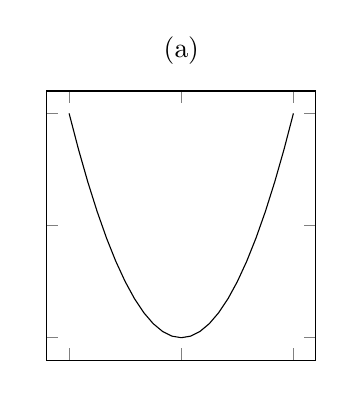
\begin{tikzpicture}
    \begin{axis}[
        width=5cm,
        height=5cm,
        title={(a)},
        yticklabels={,,},
        xticklabels={,,},
      ]
      \addplot[domain=-1:1] {x^2};
    \end{axis}
  \end{tikzpicture}%
  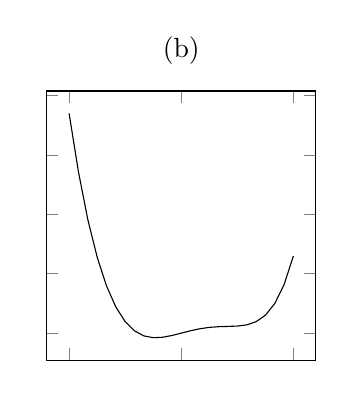
\begin{tikzpicture}
    \begin{axis}[
        width=5cm,
        height=5cm,
        title={(b)},
        yticklabels={,,},
        xticklabels={,,},
      ]
      \addplot[domain=-1:1] {x - 5*x^3 + 5*x^4 + 1.6*x^5};
    \end{axis}
  \end{tikzpicture}%
  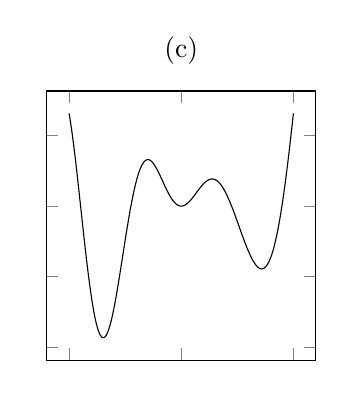
\begin{tikzpicture}
    \begin{axis}[
        width=5cm,
        height=5cm,
        title={(c)},
        yticklabels={,,},
        xticklabels={,,},
      ]
      \addplot[domain=-1:1, samples=1000] {sin(deg(7*x))*(x^4 - x^2 + x)};
    \end{axis}
  \end{tikzpicture}%
  \begin{tikzpicture}
    \begin{axis}[
        width=5cm,
        height=5cm,
        title={(d)},
        yticklabels={,,},
        xticklabels={,,},
      ]
      \addplot[solid, mark=none]
        table[x expr=\coordindex+1, y index=0] {plots/energy_landscape.csv};
    \end{axis}
  \end{tikzpicture}%
  \caption{Convex functions like the one shown in (a) can be minimized extremely
  efficiently even over high-dimensional domains. While the second example (b)
  is not convex anymore, it is smooth and has a unique minimum. Therefore local
  iterative methods will do an excellent job and converge quickly to the
  minimum. Function (c) is still smooth, but has several minima. Depending on
  where we position the starting point, iterative gradient methods might get
  stuck in one of the two local minima on the right and not find the global
  minimum on the left. The fourth function (d) is not even once differentiable
  and has numerous minima. We can only use heuristics and hope to get close to
  the true minimum.}
\label{fig:samplefuncs}
\end{figure}

The domain of our spin lattice optimization problem is a~$2 N_x N_y
N_z$-dimensional space. Even for relatively small lattices optimization in such
a high-dimensional space is generically hard. Unfortunately, it appears
completely hopeless to efficiently implement the gradient or even Hessian of the
Hamiltonian~\eqref{hamiltonian}. Moreover, it is hard to develop intuition about
how the energy landscape looks like, not only because we can barely visualize
anything in more than three dimensions. It appears certain, however, that it
will include a vast number of local minima with rough hills and valleys. It is
likely to be a higher-dimensional equivalent of plot~(d) in
\figref{fig:samplefuncs}. All of this is bad news for efficient iterative
optimization methods and we have to fall back to heuristics.

Our only option is to sample the search space preferably in a smart and
structured way and hope to capture the minimum within reasonable computation
time. This is precisely what simulated annealing is about. It merely consist of
a sampling strategy like the Metropolis algorithm that involves some randomness
and tries to gradually settle in states of lower and lower energy. We will
discover the Metropolis algorithm in the next section. As was the case for
integration, this is horrifically inefficient. By now we understand why Monte
Carlo techniques should only be considered once everything else failed or proved
intractable.
%
%%%%%%%%%%%%%%%%%%%%%%%%%%%%%%%%%%%%%%%%%%%%%%%%%%%%%%%%%%%%%%%%%%%%%%%%%%%%%%%%
\section{The Metropolis algorithm}\label{sec:metropolis}
%%%%%%%%%%%%%%%%%%%%%%%%%%%%%%%%%%%%%%%%%%%%%%%%%%%%%%%%%%%%%%%%%%%%%%%%%%%%%%%%
%
The name \newterm{simulated annealing} already hints towards thermodynamic
processes, which we identified to be a key feature of our system, but were not
yet able to bake it into the model. Clearly any real system at finite
temperature is not completely static, \ie{} stuck in a fixed state~$\pi \in
\Pi$, but it is constantly subject to thermal fluctuations. The Metropolis
algorithm, which is the core part of the simulated annealing algorithm we will
describe later, is designed to mimic real world systems at finite temperature
and will take care of thermal fluctuations. That implies that we will not seek
to find a single best state~$\pi \in \Pi$, but only consider thermal averages of
observables over many configurations. To fully understand and appreciate the
Metropolis algorithm and its ties to physics, we need some basic concepts from
statistical physics.

\subsection{Statistical physics in a nutshell}

In macroscopic many body systems such as gases or condensed matter at finite
temperature, we are often not interested in every single detail of that system
at a given moment in time. For example, we do not want to know the position and
velocity as well as rotational and vibrational modes of each single molecule in
a piston. Sensible observables are typically some sort of macroscopic averages
like the volume, temperature or pressure of the gas. For a solid we might be
interested in its specific heat, conductivity or susceptibility rather than the
joint many body wave function of all electrons. Statistical physics provides a
sound and rigorous way to define those averages.

Instead of working with the complete microstates, in our case the elements
of~$\Pi$, directly, we only talk about the probability~$P_{T}(\pi)$ that the
system is in a certain state~$\pi \in \Pi$ at temperature~$T$. To this end we
imagine a large ensemble of exact replicas of the system and observe them all at
the same time figuratively counting how often each microstate occurs. Starting
from the assumption that in a closed system in equilibrium each microstate~$\pi$
is equally likely, we can derive the so called \newterm{canonical ensemble}. It
states that the probability of a non-closed system in equilibrium at finite
temperature~$T$, \eg{} via contact to a large heat bath, to be found in
state~$\pi$ is
%
\begin{equation}\label{boltzmann}
  P_{T}(\pi) = \frac{\exp \left(- \frac{H(\pi)}{k_B T}\right)}
  {\sum_{\pi \in \Pi} \exp \left(- \frac{H(\pi)}{k_B T}\right)}\:.
\end{equation}
%
This is also referred to as the \newterm{equilibrium Boltzmann distribution}
with~$k_B$ being the Boltzmann constant. For a finite configuration
space~$P_T(\pi)$ are discrete probabilities that add up to one by construction.
The normalizing factor
%
\begin{equation}
  Z := \sum_{\pi \in \Pi} \exp(-\beta H(\pi))
\end{equation}
%
in~\eqref{boltzmann} is called \newterm{partition function}. Here we introduced
the common shortcut~$\beta := {(k_B T)}^{-1}$. In our case,~$\Pi$ consists of
infinitely many states and the summation in the partition function has to be
replaced by an integral
%
\begin{equation}
  Z := \int_{\Pi} \exp(-\beta H(\pi)) \sucd{\mu}_{\Pi}(\pi)\:,
\end{equation}
%
where the measure~$\mu_{\Pi}$ depends on the configuration space. In our system
it is a product measure of the standard measure on~$S^2$, but the mathematical
details are not important for the further treatment in this report. Note that we
will always consider the equilibrium Boltzmann distribution for a fixed
temperature~$T$ and sometimes drop the subscript~$T$ and simply denote it
by~$P$.

The equilibrium Boltzmann distribution~\eqref{boltzmann} tells us that
configurations with lower energy are exponentially more likely than
configurations with higher energy. Furthermore, this effect is most pronounced
at low temperatures. If~$T$ is large, states with higher energy still occur with
a decent probability compared to the minimizing state. On the other hand, for~$T
\to 0$ basically only the state with minimal energy has a non-zero probability.
Both facts match our intuition. At high temperatures, thermal fluctuations are
large and the system can visit many different microstates. At zero temperature
we expect the system to settle in the ground state.

In a probabilistic description, the energy or magnetization of one single
specific configuration looses its significance. Instead we measure expectation
values of observables. For an observable~$\map{\cO}{\Pi}{\bR}$ we compute the so
called \newterm{thermal average}
%
\begin{equation}\label{thermavgsum}
  \avg{\cO} := \frac{1}{Z} \sum_{\pi \in \Pi} \cO(\pi) \exp(- \beta H(\pi))\:,
\end{equation}
%
hence we average over all states weighted by their probability at a given
temperature. For a continuous state space this becomes
%
\begin{equation}\label{thermavgint}
  \avg{\cO} := \frac{1}{Z} \int_{\Pi} \cO(\pi) \exp(- \beta H(\pi))
    \sucd{\mu}_{\Pi}(\pi)\:.
\end{equation}
%
In our case the observables we are primarily interested in are the
energy~$\avg{H}$ and the three components of the magnetization~$\avg{\M} =
\avg{\sum_{\r \in \Sigma} \S_{\r} / \abs{\Sigma}}$.

One question immediately poses itself: How could we possibly compute the
high-dimensional integral in~\eqref{thermavgint} for our specific situation?
Even for finite configuration spaces the sum in~\eqref{thermavgsum} would
contain extraordinarily many terms. If each lattice site could only be in two
states, up or down, already on a small~$10^3$ lattice we would have to sum
up~$2^{1000} \approx 10^{300}$ configurations. This is far beyond the
possibilities of any machine imaginable today. The large dimensionality of the
problem renders it a good fit for Monte Carlo methods.
Indeed~\eqref{thermavgint} bears striking resemblance to~\eqref{probform}. The
standard measure on~$S^2$ can be derived from the Lebesgue measure~$\lambda^3$
on~$\bR^3$ and~\eqref{boltzmann} by construction can be interpreted as a
probability density function~$p$ on~$\Pi$. It assigns almost no weight to
configurations with high energy. As a consequence they will not contribute much
to the integral. The thermal average obviously calls for importance sampling
%
\begin{equation}\label{thermavgapprox}
  \avg{\cO} \approx \frac{1}{N} \sum_{i = 1}^N \cO(\pi_i)\:,
\end{equation}
%
where~$\pi_i$ are independent samples drawn from the Boltzmann
distribution~$P_T$. Finally we see how Monte Carlo integration enters the
picture.

\subsection{Generating random configurations}\label{subsec:random}

The challenge is to generate independent random samples following the Boltzmann
distribution~\eqref{boltzmann}. Generating a uniformly random configuration is
relatively easy, although there is one major pitfall one has to look out for.
The strategy is of course to pick a uniformly random spin at each vertex of the
grid. We assume that the programming language of choice has efficient built in
routines for pseudo random numbers following common distributions such as the
uniform, normal or exponential distribution.

Some programmers claim to generate uniformly random elements of~$S^2$ in the
following way. They generate three random numbers~$x,y,z \sim \cU_{[-1,1]}$ and
then normalize the resulting vector~$(x,y,z) / \sqrt{x^2 + y^2 + z^2}$.
While~$(x,y,z)$ in this case is uniformly distributed on the cube~$[-1,1]^3$, by
simply projecting all points onto the sphere~$S^2 \subset [-1,1]^2$, the points
that were originally generated outside the sphere, \ie{} in~$[-1,1]^3 \setminus
B^3$, are unevenly distributed. Here the unit ball~$B^3$ is the interior
of~$S^2$. The corners of the cube host more points than the areas where the
sphere actually touches the faces of the cube and thus we expect more points in
a small neighborhood around~$(1,1,1)/\sqrt{3}$ than around~$(0,0,1)$.

There are several ways to mitigate this effect. One is to discard all
points~$(x,y,z)$ with length greater than one and redraw new points in the cube
until they fall inside the sphere. We do not recommend this method, because of
its inefficiency. In three dimensions we have~$\lambda^3([-1,1]^3) =
8$,~$\lambda^3(B^3) = 4 \pi / 3$ and thus
%
\begin{equation}
  \frac{\lambda^3([-1,1]^3 \setminus B^3)}{\lambda^3([-1,1]^3)} \approx 0.476\:,
\end{equation}
%
\ie{} one would have to discard almost every second candidate. The ratio becomes
ever larger in higher dimensions. A slightly better way is make use of the fact
that~$S^2$ is a two-dimensional manifold, thus can be parameterized by only two
real numbers. One can independently draw~$x,y \sim \cU_{[-1,1]}$, discard and
redraw them if~$x^2 + y^2 > 1$ and otherwise return
%
\begin{equation}
  \begin{pmatrix}
    2 x \sqrt{1 - x^2 - y^2} \\
    2 y \sqrt{1 - x^2 - y^2} \\
    1 - 2 (x^2 + y^2)
  \end{pmatrix} \:,
\end{equation}
%
which results in a uniform distribution on the sphere. This is a slight
improvement, because we only discard the fraction
%
\begin{equation}
  \frac{\lambda^2([-1,1]^2 \setminus B^2)}{\lambda^2([-1,1]^2)} \approx 0.215\:,
\end{equation}
%
but still not optimal. Interestingly, the original
method~$(x,y,z)/\norm{(x,y,z)}$ works if we draw~$x,y,z$ independently from a
normal distribution with zero mean. The downside of this approach is that the
generation of normally distributed random numbers is slightly slower than
uniformly distributed ones.

Finally, let us describe the method we used. In the simulation itself we prefer
the redundant representation as three-dimensional vectors, because it simplifies
the computation of dot and cross products as well as projections onto coordinate
planes. Nevertheless for the generation of uniformly random spins on~$S^2$ it is
advantageous to work in spherical coordinates~$(\phi, \theta) \in [0,2\pi)
\times [0,\pi)$. The next pitfall is already waiting for us. Uniformly
chosen~$\phi$ and~$\theta$ will also \emph{not} result in a uniform distribution
on~$S^2$. The density of points would be larger near the north and south pole,
\ie{} for~$\theta \approx 0$ and~$\theta \approx \pi$, than near the
equator~$\theta \approx \pi/2$. The correct procedure is the following:
%
\begin{enumerate}
  \item Draw~$z \sim \cU_{[-1,1]}$ and~$\phi \sim \cU_{[0,2\pi)}$.
  \item Compute~$r_{xy} = \sqrt{1 - z^2}$.
  \item The vector~$(r_{xy} \cos(\phi), r_{xy} \sin(\phi), z)$ is a sample
    from~$\cU_{S^2}$.
\end{enumerate}
%
Here we make use of the fact that the~$z$ component, \ie{}~$\cos(\theta)$, of
uniformly distributed points on~$S^2$ is uniformly distributed on~$[-1,1]$. The
azimuthal angle~$\phi$ is also uniformly distributed on~$[0,2\pi)$. The~$x$
and~$y$ components are then computed such that the resulting vector has unit
length. Note that for all intervals above it does not matter whether we include
the end points or not, because they constitute a null set with respect to the
Lebesgue measure. In our benchmarks the latter method was almost a factor two
faster than all other presented options.

By now we have at least clarified how to generate a uniformly random
configuration~$\pi \sim \cU_{\Pi}$, which we will need later. The Metropolis
algorithm is a recipe on how to generate configurations drawn from the
equilibrium Boltzmann distribution if we have access to uniformly random
samples. The mathematical tool for this recipe to succeed is the theory of
Markov chains.

\subsection{Markov chains}

The crucial idea is to not create each random sample of the equilibrium
Boltzmann distribution completely from scratch, but to slowly work towards more
likely configurations. If we simply pick a uniform random configuration, we can
only evaluate its energy once it has been generated. It would take a huge number
of samples to figure out which energies are relatively high and therefore
unimportant, or relatively low and therefore contribute a lot. Even if we knew
the energy range up front, we could not generate configurations in a certain
energy range from scratch, but only decide after we have generated them.

The cure for this problem are so called \newterm{Markov chains}. In a Markov
chain we start at any configuration~$\pi_0$ and modify it to transition to the
next one~$\pi_1$. Then we continue from there, which yields the following
sequence or chain
%
\begin{equation}
  \xymatrix{\pi_0 \ar[r]^{\phi} &\pi_1 \ar[r]^{\phi} &\pi_2 \ar[r]^{\phi}
  &\;\cdots}
\end{equation}

The transition procedure, which we denoted by~$\phi$, has to fulfill two
requirements. At some point we want configuration~$\pi$ to occur in the chain
with probability~$P_T(\pi)$, \ie{} it has to actually sample the equilibrium
Boltzmann distribution. The second requirement stems from the fact that for
Monte Carlo integration to work we need independent samples. Since~$\pi_{i}$ now
clearly depends on~$\pi_j$ for~$j < i$, we have to make sure that~$\phi$
modifies each state enough to render~$\pi_{i+1}$ practically independent
of~$\pi_i$. We can characterize~$\phi$ by the probability with which it
transforms state~$\pi$ into state~$\pi'$. For each pair of states~$\pi, \pi' \in
\Pi$ we denote the transition probability by~$\T(\pi \to \pi')$. Proper
transition probabilities have to fulfill
%
\begin{equation}\label{probprop}
  \sum_{\pi' \in \Pi} \T(\pi' \to \pi) = 1 \qqtxtqq{or}
  \int_{\Pi} \T(\pi' \to \pi) \sucd{\mu}_{\Pi}(\pi') = 1
\end{equation}
%
meaning that starting from~$\pi$ the system has to go to \emph{some} other state
in the configuration space with probability~$1$. Furthermore we require~$\T(\pi
\to \pi') \ge 0$ for all~$\pi, \pi' \in \Pi$.

\subsubsection{State transitions of the three-dimensional spin lattice}

For illustration purposes let us explain what the transition process~$\phi$ will
look like in our specific example. The simplest way to modify a state~$\pi \in
\Pi$ is to pick one of the spins~$\S_{\r} \in S^2$ and change it. Since we have
no indicators yet as to which spin we should change and how to modify it to
bring the new state close to a sample from the Boltzmann distribution, we follow
the Monte Carlo scheme and select the position~$\r \in \Sigma$ as well as the
new spin~$\S'_{\r}\in S^2$ uniformly at random, respectively. Obviously, flipping
one spin out of many does not yet result in an independent state. In fact the
correlation between the two configurations would be almost one. Thus~$\phi$ has
to consist of a little more than just changing one spin. Henceforth let us call
the action of changing one spin an \newterm{update}.

Instead of a single update, we change many spins and we change them often.
Successively updating~$\abs{\Sigma} = N_x N_y N_z$ random vertices is called one
\newterm{lattice sweep} or just \newterm{sweep}. The transition~$\phi$ from one
configuration to the next will consist of~$\Nsweep \in \bN$ many lattice sweeps.
Thus, between two successive configuration each lattice site has been
updated~$\Nsweep$ many times on average, see \figref{fig:update}. The exact
number~$\Nsweep$ has to be determined by careful analysis such that~$\pi_{i+1}$
is independent of~$\pi_i$. We will come to this delicate business in
\secref{sec:analysis}. In our simulation we will measure time by the number of
lattice sweeps. This measure is called Monte Carlo time and one sweep is
referred to as a Monte Carlo step. One has to be careful not to confuse
consecutive configurations in the Markov chain, which are separated by multiple
sweeps and intermediate configurations that are separated by a single sweep. We
will hardly ever consider different configurations within one sweep, \ie{}
separated by less than~$\abs{\Sigma}$ updates.

Apparently, if we simply keep updating spins in that fashion, each transition
will have the same probability and we only generate one uniformly random sample
of~$\Pi$ after the other instead of drawing from the Boltzmann distribution. By
carefully selecting which updates actually are allowed to happen and which we
reject without any changes to the current state, we can tune the transition
probabilities to our liking.

\begin{figure}[H]
  \centering
  \begin{tikzpicture}
    \draw[thick] (0,0) -- +(0.5,0) node[pos=0, left] {$\pi_i$};
    \draw[->,>=latex, thick] (13.3,0) -- +(0.5,0) node[pos=1, right] {$\pi_{i+1}$};
    \begin{scope}[xshift=6cm]
      \config{}
    \end{scope}
  \end{tikzpicture}
  \caption{To render state~$\pi_{i+1}$ independent of state~$\pi$, we
  perform~$\Nsweep$ sweeps, each consisting of~$\abs{\Sigma} = N_x N_y N_z$
  updates.}
\label{fig:update}
\end{figure}

\subsubsection{Transition probabilities}

Let~$P_i(\pi)$ be the probability that at the~$i$-th step of
the chain we are in state~$\pi$. This probability can be computed recursively.
What is the probability that at step~$i+1$ we are in state~$\pi$? There are
basically two ways we could end up there. Either we were in a different
state~$\pi'$ at the~$i$-th step and hit the transition probability~$\T(\pi' \to
\pi)$, or we have already been in~$\pi$ and stayed there, which happens with
probability~$\T(\pi \to \pi)$. Those can be combined into
%
\begin{equation}\label{master}
  P_{i+1}(\pi) = \sum_{\pi' \in \Pi} P_i(\pi') \T(\pi' \to \pi) \qqtxtqq{or}
  P_{i+1}(\pi) = \int_{\Pi} P_i(\pi') \T(\pi' \to \pi) \sucd{\mu}_{\Pi}(\pi')\:.
\end{equation}
%
Let us refactor this expression, using only the summation notation, because it
is simpler and can trivially be transformed into the continuous version.
With~\eqref{probprop}, we find
%
\begin{align}\label{masterlong}
  P_{i+1}(\pi) &= \sum_{\pi' \in \Pi} P_i(\pi') \T(\pi' \to \pi) +
    P_i(\pi) \biggl(1 - \sum_{\pi' \in \Pi} \T(\pi \to \pi')\biggr)\nonumber \\
  &= P_i(\pi) + \sum_{\pi' \in \Pi}
    (P_i(\pi') \T(\pi' \to \pi) - P_i(\pi) \T(\pi \to \pi'))\:.
\end{align}
%
In this form we can interpret the first term of the sum as all the ways we can
enter state~$\pi$ at step~$i+1$ and the second term as all the ways we can leave
state~$\pi$ in step~$i+1$. This form will prove helpful in a moment.

Now we aim at tuning the transition probabilities such that~$\lim_{i \to \infty}
P_i = P$, \ie{} the probabilities in~\eqref{master} converge to a stationary
distribution that agrees with the Boltzmann distribution~\eqref{boltzmann}. In a
stationary distribution, the probability of entering a certain state has to be
equal to the probability of leaving that state. If we entered a state more often
than we left it or vice versa, the distribution would clearly not be stationary.
Mathematically this signifies that we can tune the transition probabilities such
that the terms of the sum in~\eqref{masterlong} cancel each other out. In the
limit~$i \to \infty$, where~$P_i(\pi) = P(\pi)$ for all states~$\pi \in \Pi$, we
thus find
%
\begin{equation}\label{detbal}
  P(\pi') \T(\pi' \to \pi) = P(\pi) \T(\pi \to \pi')\:.
\end{equation}
%
This condition is called \newterm{detailed balance} and is a key feature of
Markov chains. We can interpret it as reversibility of the transition
process~$\phi$. Going from~$\pi$ to~$\pi'$ is equally likely as the other way
round.

For completeness, let us mention that the second key requirement for Markov
chains to work properly is \newterm{ergodicity}. Ergodicity says that each state
must be reachable from every other state in a finite number of steps. We are
not going to elaborate on the theoretical importance of this property, but only
point out that ergodicity is clearly fulfilled in our specific model, because we
have to change a maximum of~$N_x N_y N_z$ spins and each possible spin flip has
non-zero probability at finite temperature. One can show that if detailed
balance and ergodicity are fulfilled, the Markov chain is guaranteed to converge
to a stationary distribution.

\subsubsection{The Metropolis algorithm}

The ratio of the transition probabilities in the stationary distribution reveal
another interesting aspect
%
\begin{equation}
  \frac{\T(\pi \to \pi')}{\T(\pi' \to \pi)} = \frac{P(\pi')}{P(\pi)} =
  e^{-\beta (H(\pi') - H(\pi))} =: e^{-\beta \Delta H}\:.
\end{equation}
%
Thus the transition probabilities depend only on the energy difference of the
two states in question. In particular there is no memory of previous states. At
each step we can decide the transition probability purely from the current and
the proposed successor configuration. This property is our main guidance in
engineering the transition probabilities. One rather obvious choice is given by
%
\begin{equation}
  \T(\pi \to \pi') = \min(1, e^{-\beta (H(\pi') - H(\pi))})\:.
\end{equation}
%
Those are the so called \newterm{Metropolis} (or \newterm{Metropolis-Hastings})
transition probabilities. The whole Markov chain Monte Carlo integration for
thermodynamic systems like ours using the Metropolis transition probabilities is
simply called \newterm{Metropolis algorithm} or \newterm{Metropolis-Hastings
algorithm}. There are also other plausible choices for the transition
probabilities, for example the so called \newterm{Heatbath}, \newterm{Glauber},
or \newterm{overrelaxation} algorithms, but we will only discuss and implement
the Metropolis algorithm.

Now that we know the transition probabilities, we can bake them into our state
transition procedure~$\phi$. Recall that~$\phi$ consists of~$\Nsweep$ lattice
sweeps, each of which performs~$\abs{\Sigma}$ random updates of single spins.
Each time we have selected a spin~$\S_{\r}$ from the current configuration~$\pi$
for an update, we will first generate its potential replacement~$\S'_{\r} \sim
\cU_{S^2}$, which would lead to state~$\pi'$. But now we only actually perform
the update, if
%
\begin{equation}
  \T(\pi \to \pi') \ge p, \quad \text{where } p
    \text{ is a sample from } \cU_{[0,1)}\:.
\end{equation}
%
Note that this is the only time we consider configurations that are separated by
just one update. We do not accept or reject full lattice sweeps or even
applications of~$\phi$ but every single update within every sweep. Thereby we
abide to the desired transition probabilities in each update, thus in each sweep
and eventually also in each complete transition~$\phi$.

\subsubsection{Thermalization and the start configuration}

Theoretically a Markov chain goes on forever, traversing the configuration
space, each time choosing the successor state at random according to the
transition probabilities. Given detailed balance and ergodicity, after
sufficiently many steps, we have converged to a stationary distribution and each
new state can be considered an independent sample from the equilibrium Boltzmann
distribution. Those initial steps before the distribution becomes stationary are
called \newterm{thermalization}. The close ties to thermodynamics are obvious,
where a system can only be treated statistically, if it is in thermal
equilibrium, \ie{} after it has thermalized. Hence, before we can actually use
the states~$\pi_i$ as independent samples of the Boltzmann distribution to
estimate thermal averages via~\eqref{thermavgapprox}, we have to
perform~$\Ntherm$ lattice sweeps to equilibrate the system. Henceforth the
time~$t$ is measured by the number of lattice sweeps we have performed. While
detailed balance and ergodicity guarantee that there is some finite~$\Ntherm \in
\bN$, the precise value depends on a number of factors.

First of all it depends on the start configuration. In lattice models like ours
the two most commonly used options are a \newterm{hot start} or a \newterm{cold
start}. In a hot start we initialize the first state uniformly at random~$\pi_0
\sim \cU_{\Pi}$. Practically that means that we initialize each spin~$\S_{\r}$
for~$\r \in \Sigma$ independently uniformly at random~$\S_{\r} \sim \cU_{S^2}$
as discussed in subsection~\ref{subsec:random}. It is called hot start, because
in the limit~$T\to \infty$ the Boltzmann distribution becomes a uniform
distribution and each state is equally likely. Hence at infinite temperature a
hot start already follows the Boltzmann distribution and the system is in
thermal equilibrium from the very beginning. In a cold start all spins are
chosen in the same direction, possibly parallel to the external magnetic field,
which corresponds to a global minimum of the Hamiltonian including only direct
exchange and the Zeeman energy at zero temperature.

Secondly, the thermalization time varies with temperature. We have already seen
that at high temperatures almost all transitions have a decent probability and
we can explore many states in a short time, guiding the system into equilibrium
faster. At very low temperatures the Boltzmann distribution is highly localized,
peaked at low energy states and we will have to reject many proposed successors
before we discover the probable configurations. Generally this yields a long
thermalization time for low temperatures. We will experience this tendency quite
forcefully in \chapref{chap:2}, when we analyze our specific model.

Thirdly, the system size plays a crucial role. The equilibration time
unsurprisingly grows directly with the system size. This can be understood
easily simply from the fact that in a large system it takes longer for all parts
of it to communicate with each other and find a joint equilibrium state. We will
discuss in the next section, how one can detect when the system is fully
equilibrated. From here on we will consider~$\pi_0$ to be the initial
configuration and~$\pi_1$ to be the first configuration after thermalization,
\ie{} the first one that can actually be used to compute thermal averages.
Afterwards all following configurations are separated by~$\Nsweep$ sweeps.

\subsection{Summary and pseudocode}

The ultimate goal of the Metropolis algorithm is to estimate observables such as
the energy or the magnetization at fixed temperature~$T$ and external field~$B$.
Therefore it has to output the collection of desired observables, which we
denote generically by~$\cO$, for~$N$ independent samples of the Boltzmann
distribution. Let us now put all the pieces together and lay out a pseudo code
for the Metropolis algorithm at fixed temperature~$T$ and external field~$B$ in
Algorithm~\ref{alg:metropolis}. The full metropolis algorithm can be depicted
schematically as

\begin{equation}
  \xymatrix{%
    \text{initialize} \ar[d]
      &\text{save } \cO(\pi_1)
      &\text{save } \cO(\pi_2)
      && \text{save } \cO(\pi_N) \\
    \pi_0 \ar[r]^{\Ntherm}_{\text{sweeps}}
    & \pi_1 \ar[r]^{\Nsweep}_{\text{sweeps}} \ar[u]
    & \pi_2 \ar[r]^{\Nsweep}_{\text{sweeps}} \ar[u]
    & \cdots \ar[r]^{\Nsweep}_{\text{sweeps}}
    & \pi_N \:. \ar[u]
  }
\end{equation}

The starting configurations~$\pi_0$ can technically be chosen as one pleases, we
always use a hot start~$\pi_0 \sim \cU_{\Pi}$. The initial state~$\pi_0$ is not
used in computing thermal averages. We have to choose~$\Ntherm$ large enough for
the system to equilibrate, \ie{} reach a stationary distribution, and~$\Nsweep$
large enough to render subsequent configurations of the Markov chain
uncorrelated. The number of configurations~$N$ determines the error~$\sim
1/\sqrt{N}$ of the final estimate
%
\begin{equation}
  \avg{\cO} = \frac{1}{N} \sum_{i=1}^N \cO(\pi_i) \:.
\end{equation}
%
In practice the error estimate for this value~$\avg{\cO}$ is computed by the
jackknife method as described earlier in subsection~\ref{integration}.

\begin{algorithm}
  \caption{Metropolis algorithm}\label{alg:metropolis}
  \begin{algorithmic}[1]
    \Require{Initialize the spin lattice, \eg{} with a hot start~$\pi_0 \sim
    \cU_{\Pi}$.}
    \Statex
    \Procedure{metropolis}{$\pi_0$, $T$, $B$} \Comment{$T, B$ are fixed}
      \For{$i$ from~$1$ to~$\Ntherm$} \Comment{thermalization}
        \State \textsc{sweep}($\pi_0$)
      \EndFor
      \State set $\pi_1 := \pi_0$
      \State save~$\cO(\pi_1)$
      \For{$i$ from~$1$ to~$N-1$}
        \State set $\pi_{i+1} :=$ \textsc{next\_config}($\pi_i$)
        \State save~$\cO(\pi_{i+1})$
      \EndFor
    \EndProcedure
    \Statex
    \Function{next\_config}{$\pi$}
      \For{$j$ from~$1$ to~$\Nsweep$}
        \State \textsc{sweep}($\pi$)
      \EndFor
      \State \Return{$\pi$}
    \EndFunction
    \Statex
    \Procedure{sweep}{$\pi$} \Comment{\textsc{sweep} modifies~$\pi$}
      \For{$i$ from~$1$ to $N_x N_y N_z$}
        \State draw $\r \sim \cU_{\Sigma}$
        \State draw $\S' \sim \cU_{S^2}$
        \If{$\min\bigl(1, \exp(- \beta \Delta H)\bigr) >
          \mathrm{rand}(0,1)$}
            \State replace~$\S_{\r} \in \pi$ by~$\S'_{\r}$
        \EndIf
      \EndFor
    \EndProcedure
  \end{algorithmic}
\end{algorithm}

%
%%%%%%%%%%%%%%%%%%%%%%%%%%%%%%%%%%%%%%%%%%%%%%%%%%%%%%%%%%%%%%%%%%%%%%%%%%%%%%%%
\section{Simulated annealing}\label{sec:siman}
%%%%%%%%%%%%%%%%%%%%%%%%%%%%%%%%%%%%%%%%%%%%%%%%%%%%%%%%%%%%%%%%%%%%%%%%%%%%%%%%
%
In \secref{sec:model} we formulated our initial goal as an optimization problem.
However, in everything that followed the general introduction of Monte Carlo
methods in \secref{sec:mctheory} was concerned with integration only. We
discovered that a truly thermodynamic treatment does not allow us to distinguish
a single energetically favored state, but necessitates in thermal averages which
we approximate by Monte Carlo integration using importance sampling. Proper
samples are provided by a Markov chain with Metropolis transition probabilities.
Hence, we can now observe thermodynamic quantities such as the energy or
magnetization of the spin lattice in equilibrium at fixed temperature~$T$ and
magnetization~$B$. A certain notion of minimizing the energy is implicit,
insofar as we are always more likely to accept transitions towards lower energy
states. While we are now able to scan the whole phase space spanned by~$B$
and~$T$ and partition it into regions with similar properties, we cannot
dynamically observe phase transitions.

Imagine a rough energy landscape similar to the one depicted in plot~(d) of
\figref{fig:samplefuncs}. If we fix~$T$ and~$B$ from the very beginning, even
the Markov chain might get stuck in a certain region of the configuration space
or is extremely unlikely to find specific parts of it. In physical systems such
rare configurations that are hard to reach do indeed emerge. If we start at a
high temperature, however, the Markov chain will definitely sample most of the
configuration space with a decent probability. If we then slowly decrease the
temperature, it has a substantially better chance of annealing into such an
interesting portion of~$\Pi$. This is the whole idea behind simulated annealing.
Instead of fixing~$T$ and~$B$ once and for all, we might start at at fixed point
in the phase space, wait until the system has thermalized and compute~$N$
configurations of the Markov chain for the starting~$T$ and~$B$ like before. But
instead of stopping right there and initializing a whole new run, one
changes~$T$ or~$B$ by a tiny amount, discards some sweeps for thermalization and
records another~$N$ configurations of the Markov chain. It is essentially a
wrapper around the Metropolis algorithm that keeps building up the Markov chain
with intermediate changes of the parameters. This method allows us to trace out
paths within the phase space. It can be used to observe phase transitions or
reach configurations that are hard to find by fixing the position in phase space
from the very beginning.

For completeness let us explain why simulated annealing was introduced as an
optimization method. Imagine our objective was actually to minimize the
Hamiltonian. While there are no iterative or local methods to minimize it
directly, we have found that the Metropolis algorithm efficiently samples the
configuration space with a favor for low energy states, especially for low
temperatures. Thus if we start at a high temperature and slowly decrease it, the
Markov chain will tend to concentrate around lower and lower energies. If we are
lucky and the energy landscape is not too rough, there is a good chance it will
eventually settle in the absolute minimum for~$T \to 0$. Apparently we need to
\emph{anneal} the system, because starting with~$T=0$, the Metropolis algorithm
will never accept any changes towards higher energies at all and we are bound to
get stuck in the nearest local minimum. Moreover, we cannot bridge or tunnel
large barriers, because any single update can only change the energy by a fixed
amount.

%
%%%%%%%%%%%%%%%%%%%%%%%%%%%%%%%%%%%%%%%%%%%%%%%%%%%%%%%%%%%%%%%%%%%%%%%%%%%%%%%%
\section{Analysis and statistics}\label{sec:analysis}
%%%%%%%%%%%%%%%%%%%%%%%%%%%%%%%%%%%%%%%%%%%%%%%%%%%%%%%%%%%%%%%%%%%%%%%%%%%%%%%%
%
In the previous sections we discussed the Metropolis algorithm and provided a
pseudocode which should make it fairly easy to implement. However, we issued
quite a few warnings without yet giving specific instructions on how to stay on
the safe side of things. How should one choose the thermalization time~$\Ntherm$
and how do we know whether the system is in equilibrium? How large
does~$\Nsweep$ have to be such that consecutive configurations of the Markov
chain can be considered independent? In this section we try to answer these
questions or at least provide some practical guidelines.

\subsection{Thermalization}

Equilibration is a sensitive and often underestimated topic. It is by far not
sufficient to let ``a few sweeps'' go by after a hot start, even at high
temperatures. In the literature one can find guidelines that suggest that the
thermalization time should be at least~$15-20$\% of the total runtime. The total
runtime, as always measured in Monte Carlo time, \ie{} the number of lattice
sweeps, is given by~$\Ntherm + N\cdot \Nsweep$. Such estimates, while helpful
for getting an idea of the order of magnitude, often lure scientists into
blindly allocating~$20$\% of the overall runtime for equilibration and feel
safe. This is plain wrong and indefensible. Despite all the factors that go into
the thermalization time, the number of sweeps in between configurations and the
overall number of configurations one chooses to compute are not among them. How
could one expect the thermalization time to decrease only because we stop the
Markov chain after a few configurations? Those are just the most obvious flaws
in such recommendations. Besides the system size, the temperature and the start
configuration, the equilibration time also differs for various observables and
of course for different systems and models. We cannot expect to find a solution
without closely analyzing the specific final implementation of the model at
hand.

That being said, even then there is no~$100$\% foolproof recipe to
determine~$\Ntherm$ in a fully satisfying rigorous fashion. The most common
approach is to simply plot the observables one is interested in. After the
implementation is finished and before we actually start to record states of the
Markov chain, we write out \emph{all} observables we are interested in after
every single sweep beginning with the initial state. If one is interested in the
energy and the magnetization of the system, one would plot the energy and all
three components of the magnetization over Monte Carlo time~$t$, \ie{} over the
number of sweeps. In \secref{sec:results} we will do precisely that. We discover
that all observables level out over time and then fluctuate around a constant
value. This happens much later for the magnetization than for the energy. Thus
it is vital to look at such plots for all observables. The point from which
onwards all observables are basically constant, which is typically measured by
eye, is the minimal equilibration time for this specific system at a fixed point
of the phase space.

Keep in mind that in principle one has to repeat this analysis whenever one
changes the temperature, the system size, the magnetic field or any other
parameters of the model. Since hot start conditions are chosen at random, even
the exact same simulation with a different start configuration could have a
longer or shorter thermalization time. Therefore a generous additional cushion
is mandatory. Analyzing and determining~$\Ntherm$ for the whole range of
parameters one intends to simulate is the very first step after the Metropolis
algorithm has been implemented and tested for correctness.

\subsection{Autocorrelation and errors}

Another pitfall we have emphasized several times already is the necessity of
\emph{independent} samples for Monte Carlo integration to work properly. Our
samples are the states of a Markov chain with the generic characteristic that
each state is generated by modifying its predecessor. By definition the
resulting samples are not independent. However, by separating subsequent
configurations by sufficiently many Monte Carlo steps we can bring down their
correlation until they can be considered independent for all practical purposes.
We will now quantify how~$\Nsweep$ has to be chosen to guarantee such
independence. Again it does not seem too harmful to simply let a ``good amount
of'' sweeps go by in between consecutive configurations of the Markov chain, but
there is actually analytic evidence that one has to take correlations seriously.

\newterm{Autocorrelation} is \emph{the} central tool to quantify correlations of
individual states within a time series. Given an observable~$\cO$ at Monte Carlo
times~$\numlist{1}{N}$, where we start counting once the system has thermalized,
the autocorrelation function can be estimated
%
\begin{equation}\label{autocorr}
  R_{\cO}(t) := \frac{1}{\sigma^2 (N-t)} \sum_{i = 1}^{N-t}
    \cO(i) \cO(i+t) - \mu^2
\end{equation}
%
for~$t \in \numlist{0}{N-1}$, where~$\sigma^2$ is the variance and~$\mu$ the
mean of the observable~$\cO$. Note that it only makes sense to talk about the
mean and variance once we draw from a stationary distribution, \ie{} after the
system has thermalized. Since we do not have access to the true mean and
variance of observables, we have to estimate those quantities too. We use the
standard sample mean and sample variance of~$\numlist{\cO(1)}{\cO(N)}$
%
\begin{equation}\label{samplemeanvar}
  \mu = \frac{1}{N} \sum_{i=1}^N \cO(i) \qqtxtqq{and}
  \sigma^2 = \frac{1}{N-1} \sum_{i=1}^N (\cO(i) - \mu)^2
\end{equation}
%
which makes~$R_{\cO}$ a biased estimate. A few remarks are in order. First, the
observations are taken at subsequent Monte Carlo steps right after
thermalization, \emph{not} at subsequent configurations of a Markov chain.

Furthermore, note that the sum in~\eqref{autocorr} at~$t=0$ with the normalizing
factor is just the variance~$\sigma^2$, which results in~$R_{\cO}(0) = 1$. The
autocorrelation can be understood as the covariance of the sequence with a
shifted version of itself. Since we want to measure the correlation of states at
different times in the same chain this is entirely plausible. Like the
covariance, the autocorrelation can become negative. Negative autocorrelation at
time~$t$ means that large negative values of~$\cO$ at a certain time correlate
with large positive values~$t$ steps later in the chain or vice versa. The
variance in the denominator normalizes the autocorrelation to lie in~$[-1,1]$.

One major issue with the estimator~$R_{\cO}$ is due to the fact that we are
dealing with a finite sequence of measurements. The sum in~\eqref{autocorr} runs
over fewer and fewer terms the larger~$t$. However, we need a certain number of
terms in the sum to average out random fluctuations and keep the variance of our
estimate for the autocorrelation small enough. We will see in
\secref{sec:results} that autocorrelations indeed become noisy and statistically
unreliable quickly. Therefore it only makes sense to look at~$R_{\cO}$ for~$t
\ll N$. Our goal is to find the time after which the new states are not
correlated with the starting configuration anymore, \ie{} the time after which
the autocorrelation has dropped to zero or at least beneath some threshold close
to zero.

It can be shown that the autocorrelation function in Markov chain Monte Carlo
simulations generically decays like~$\exp(-t/\tau_{\cO})$, where~$\tau_{\cO}$ is
called \newterm{autocorrelation time} for observable~$\cO$. Technically this
exponential behavior only holds for~$N \to \infty$ and~$t \to \infty$ with~$t/N
\ll 1$. However, for the random walk of the Markov chain in the configuration
space this asymptotic behavior is also approximated for small~$t$ such that we
assume~$R_{\cO}(t) \approx \exp(-t/\tau_{\cO})$. The simplest but also an
inaccurate way to determine~$\tau_{\cO}$ is to plot the autocorrelation function
and find the time after which it has dropped to~$1/e$. Alternatively one can use
the integrated autocorrelation time
%
\begin{equation}\label{tauint}
  \tauint_{\cO} = \frac{1}{2} + \sum_{t=1}^{N-1} R_{\cO}(t)
\end{equation}
%
for error analysis which is typically easier to compute. As the name suggests
this definition stems from the continuous case, where for a purely exponential
autocorrelation function~$R_{\cO}(t) = \exp(t/\tau_{\cO})$ one finds
%
\begin{equation}
  \int_0^{\infty} R_{\cO}(t) \sucd{t} = \tau_{\cO}\:.
\end{equation}
%
The discrete version~\eqref{tauint} roots in the approximation
%
\begin{equation}
  \frac{1}{2} + \sum_{t=1}^{\infty} \exp \biggl( - \frac{t}{\tau} \biggr) =
    \tau + \frac{1}{12 \tau} - \frac{1}{720 \tau^3} +
    \cO\biggl( \frac{1}{\tau^5} \biggr)\:.
\end{equation}
%
Already for~$\tau = 10$ the relative error drops below~$0.1$\% and approaches
zero quickly. For all practical purposes~$\tau_{\cO} \approx \tauint_{\cO}$
if~$N$ is sufficiently large. However, due to statistical fluctuations and the
finite number of measurements they might disagree quite significantly in real
applications.

The importance of the autocorrelation time becomes obvious when one re-derives
the error of Monte Carlo integration without the assumption that the samples are
independent. Recall that for independent measurements we found that the error is
given by~$\sigma/\sqrt{N}$, with the variance~$\sigma$
from~\eqref{samplemeanvar}. If we set~$\Nsweep$ to one, \ie{} if we used every
configuration after each sweep to estimate the thermal average, the error with
correlations becomes
%
\begin{equation}\label{correrror}
  \sqrt{\frac{\sigma^2}{N}(1 + 2\tauint_{\cO})}\:.
\end{equation}
%
Thus we have to perform sufficiently many sweeps in between two usable
configurations such that each two samples are uncorrelated and the
autocorrelation function as well as the integrated autocorrelation time go to
zero. The number of sweeps in between two configurations~$\Nsweep$ should be at
least~$5 \tauint_{\cO}$ to confidently use the uncorrelated error estimate. Note
that all this delicate business of choosing independent configurations only
affects the errors and not the expectation values of observables.

Let us spend a few more words on practical matters. The finite number of
measurements limits both the computation of the autocorrelation function as well
as the sum in~\eqref{tauint} to compute the integrated autocorrelation time.
This issue could in principle be overcome by using more data points and
extrapolating to~$N\to \infty$. However, there is another even bigger practical
problem. The values of~$R_{\cO}$ become statistically unreliable even for
large~$N$ and~$t\ll N$. This typically spoils exponential fits to
determine~$\tau_{\cO}$ directly from~$R_{\cO}$. One has to find a sensitive
balance between taking into account enough values to capture the asymptotic
decay of the exponential, but not too many to avoid statistically unreliable
values spoiling the fit. The same holds true for the sum in the integrated
autocorrelation time.

In theory the sum needs to run over infinitely many values, but due to the
exponential decay one can truncate it with clear conscience. Alternatively one
can use values at small~$t$ to extrapolate to subsequent values by an
exponential fit. However, their contribution is typically small enough to
neglect them. Again, one has to choose the truncation carefully to leave out
noisy values at late times~$t$. Usually one tries to truncate the series
self-consistently such that
%
\begin{equation}\label{tauinttrunc}
  \tauint_{\cO} \approx
    \frac{1}{2} + \sum_{t=1}^{m \cdot \tauint_{\cO}} R_{\cO}(t)\:,
\end{equation}
%
where~$m$ should be roughly between~$5$ and~$6$. Even then the values for the
autocorrelation time~$\tau_{\cO}$ from an exponential fit and the integrated
autocorrelation time~$\tauint_{\cO}$, while estimating the same quantity, can
differ significantly. One should always use the more conservative of the two.

Let us summarize how to set~$\Nsweep$. We initialize the system and discard the
first~$\Ntherm$ sweeps completely. Then we record every observable of interest
after every single sweep for as many sweeps as we can within reasonable
computation times. A rule of thumb says that one should use at least~$1000
\tau_{\cO}$ values to properly estimate~$\tau_{\cO}$. Keep in mind that every
rule of thumb should be met with skepticism. With these values we compute the
autocorrelation function~\eqref{autocorr} for each observable and plot them for
small values of~$t$. One will usually see a close to exponential decay for
small~$t$ which directly transitions to noisy fluctuations, maybe even
before the autocorrelation has approached zero at all. In this case
increasing~$N$ might help. For each observable independently one then finds a
consistent truncation~\eqref{tauinttrunc} typically by a systematic search
of~$m$ and should also fit an exponential to the data on the chosen range as a
cross check. Finally, we use
%
\begin{equation}
  \tau := \max_{\cO} \tauint_{\cO}
\end{equation}
%
to determine~$\Nsweep \in [5 \tau, 6 \tau]$.

\subsection{Additional remarks}

It is important to realize that for Monte Carlo methods in general and the
Metropolis algorithm in particular one has to spend quite some time on analyzing
the system before we even start the first simulation runs. Only if~$\Ntherm$
and~$\Nsweep$ are chosen properly, can we be sure that our results make sense.
One has to carefully monitor autocorrelations starting with small systems and
high statistic and slowly transition to larger systems constantly supervising
thermalization and correlations between states.

The Metropolis algorithm is typically rather inefficient. First of all, Monte
Carlo methods are implicitly slow. Secondly, repeatedly accessing random lattice
sites, their neighbors and next-nearest neighbors prohibits efficient caching of
data. One can render the algorithm more cache friendly by updating one lattice
site after the other as they are stored in memory instead of choosing them at
random. However, for some systems this destroys ergodicity, \ie{} some states
might be unreachable from certain configurations. Despite the long computation
times we consistently used random updates.

Low acceptance rates are another crucial performance drawback. Imagine our
lattice model at low temperature and a high magnetic field. We expect the system
to settle in a fully polarized state with little thermal fluctuations. Let's say
we have reached a state where most spins are already parallel to the external
field, but just a few are still misaligned. Whenever an aligned spin is selected
the update is almost certainly rejected, because the proposal is likely to be
misaligned again, would therefore increase the energy and due to the small
temperature such moves are rejected. We might need several sweeps until one of
the still misaligned spins is selected for an update and even then the
probability that the random proposal is parallel to the magnetic field is tiny.
Thus we will have to perform many sweeps to properly align just a few lattice
sites. This will also have an impact on the autocorrelation time.

There are several alternatives and improvements to the Metropolis algorithm.
Besides choosing different acceptance probabilities like in the
\newterm{heatbath}, \newterm{Glauber} or \newterm{overrelaxation} algorithms,
there are also fundamentally different approaches such as cluster algorithms or
parallel tempering Monte Carlo (PTMC) methods. We only implemented the most
primitive version of simulated annealing possible. However, even with such a
simple setup one can observe interesting physical results. It should be a good
starting point for more sophisticated algorithms.

Furthermore, there is a phenomenon called \newterm{critical slowing}, which
implies that at certain parameter values, for example close to phase transitions
or at very low temperatures, the acceptance rate will plummet, the
autocorrelation time diverges and the evolution of the system becomes
excruciatingly slow, basically comes to a halt. This phenomenon is directly
linked to interesting physical properties of the system and hence often leads to
difficulties precisely where we want to observe it. We will not go into more
detail about how to efficiently deal with critical slowing in this report.

It is best practice to monitor the acceptance rate, \ie{} the number of accepted
updates divided by the number of proposed updates, throughout the simulation.
While the acceptance rate directly correlates with autocorrelation times in the
initial analysis, one should also monitor it it throughout the actual
simulations, for example separately for every configuration in the Markov chain.
It can be used to detect critical slowing and when error estimates might break
down.
